\documentclass{swfcthesis}

% 下面几行是用来输出封面上的水印纹。不需要的话,就注释掉。
\usepackage{pgf}
\usepackage[firstpage]{draftwatermark}
\SetWatermarkText{
\includegraphics{logolight}}
%\SetWatermarkText{西南林业大学}
\SetWatermarkScale{.4}
\SetWatermarkAngle{0}

% 「注意」
% 本模板采用的是“模块化”设计,所以下面有很多\input{}, \include{}命令。它们用到的具体文件都
% 在chapters目录中。请根据需要自行修改。

\addbibresource{sample.bib} % 参考文献

\begin{document}

\Title{金庸笔下武功详解}
\Author{周伯通}
\Advisor{王重阳}
\AdvisorTitle{祖\hspace{1em}师}

\Month{六}
\Year{一二三七}
\Univ{中华武林大学}
\Docname{本科毕业(设计)论文}
\School{全真玄门正宗学院}
\Subject{打架斗殴专业}

\AdvisorInfo{王重陽\footnote{参见维基百
    科-\href{http://zh.wikipedia.org/wiki/\%E7\%8E\%8B\%E9\%87\%8D\%E9\%99\%BD}{王重
      阳}}(1113年1月13日-1170年),原名中孚,字允卿,又名世雄,字德威,入道后改名喆,字知
  明,道号重阳子,故称王重阳。北宋末京兆咸阳(今陕西咸阳)大魏村人。中國道教分支全真道的始
  創人,后被尊为道教的北五祖之一。他有七位出名的弟子,在道教历史上称为北七真。}

\Acknowledgments{感谢师兄王重阳传我全真玄门正宗功夫,感谢段皇爷不杀之恩,感谢刘贵妃不怨旧恶,
  感谢桃花岛主黄老邪助我练就空明拳和双手互搏之术,感谢郭靖兄弟让我看《九阴真经》,感谢小龙
  女教我驭蜂之术。}

\Abstract{中國武術\footnote{参见维基百科 -
    \href{http://zh.wikipedia.org/wiki/\%E4\%B8\%AD\%E5\%9B\%BD\%E6\%AD\%A6\%E6\%9C\%AF}{中国武术}}
  是中國传统文化的重要一環。兩廣人稱為功夫,民國初期簡稱為國術(後為中央國術館正式採用之名稱);被視
  為中國文化之精粹,故又稱國粹。由於歷史發展和地域分佈關係,衍生出不同門派。中國武術主要內容包括搏擊
  技巧、格鬥手法、攻防策略和武器使用等技術。當中又分為理論和實踐兩個範疇。從實踐中帶來了有關體育、健
  身、和中國武術獨有之氣功、及養生等重要功能。理論中帶來了不少前人之經驗和拳譜記錄。因此,它体现中华
  民族对攻防技击及策略上的理解。加上經驗上積累,以自立、自強、健體養生為目標的自我運作,練習套路时顯
  示出身體動作之優美姿態。中國武術往往帶有思想冶鍊的文化特徵及人文哲學的特色、意義,對現今中國的大眾
  文化有著深遠影響\cite{wushucn}。}

\Keywords{金庸,武术,一陽指,双手互搏,空明拳,七傷拳,吸星大法,葵花宝典,九陰真經,九陽真
  經,天山六陽掌,天羅地網勢,蛤蟆功,倚天屠龍功,弹指神通,先天功,打狗棒法,全真剑法,摧心掌,降龍
  十八掌,六脈神劍,火焰刀,黯然銷魂掌,龍爪擒拿手,兰花拂穴手,龍象般若掌,劈空掌,玉女素心剑法,北
  冥神功,碧海潮生曲}

% The followings are for the English Abstract.
\enTitle{Jin Yong's Chinese Martial Arts Illustrated}
\enAuthor{Zhou Botong}
\enUniv{Chinese Kungfu University}
\enSchool{School of Taoism}
\enAbstract{Chinese martial
  arts\footnote{Wikipedia - \href{http://en.wikipedia.org/wiki/Chinese\_martial\_arts}{Chinese martial arts}}, also referred to by the Mandarin Chinese term wushu and popularly as kung fu, are a number of fighting styles that have developed over the centuries in China. These fighting styles are often classified according to common traits, identified as "families", "sects" or "schools" of martial arts. Examples of such traits include physical exercises involving animal mimicry, or training methods inspired by Chinese philosophies, religions and legends. Styles which focus on qi manipulation are labeled as internal, while others concentrate on improving muscle and cardiovascular fitness and are labeled external. Geographical association, as in northern and southern, is another popular method of categorization\cite{wushu}.}
\enKeywords{Jin Yong, Chinese martial arts, Kungfu}

%%% Local Variables: 
%%% mode: latex
%%% TeX-master: "../sample"
%%% End: 
 % 论文标题、作者、中英文摘要……等内容都在这里

%%% 不要动下面这几行
\makepreliminarypages %封面、摘要……等内容的排版
\frontmatter      %目录、表格目录、图片目录、代码目录……都属于front matter。
\tableofcontents  %目录
\listoffigures    %图片目录
\listoftables     %表格目录
\listoflistings   %代码目录

\mainmatter  %下面是主要部分了(main matter)。
             %front matter, main matter, 以及后面的back matter的不同主要体现在页码、章节的编号上。

% 下面都是论文的各个章。每一章都单独放在一个tex文件里。所有的tex文件都在chapters目录中。照猫画虎即可。
\chapter{打狗棒法}
打狗棒法\footnote{参见维基百科 -
  \href{http://zh.wikipedia.org/wiki/\%E6\%89\%93\%E7\%8B\%97\%E6\%A3\%92\%E6\%B3\%95}{《打
    狗棒法》}}乃金庸武俠小說體系中,丐幫幫主代代相傳的二大謢幫神功之一。打狗棒本來就是用來
打惡狗的竹棒,乞丐在街上討飯,經常會遇到大戶人家的惡狗,所以丐幫人物出外行乞時,手中多執一
根打狗棒,以防惡犬襲擊。打狗棒法的特點是靈活躍動,機變百出,正是由與狗搏鬥的實際生活體驗中
發展出來的技巧。

三十六路打狗棒法是丐帮开帮祖师爷所创,历来是前任帮主传后任帮主,决不传给第二个人,丐帮第三任帮主的武
功尤胜开帮祖师,他在这路棒法中更加入无数奥妙变化,数百年来,丐帮逢到危难关头,帮主亲自出马,往往便仗
这打狗棒法除奸杀敌,震慑群邪\cite{dagoubang}。

\section{棒法}

打狗棒,如图~\ref{fig:stick}所示,是丐幫幫主世代相傳的信物,丐幫中見棒如見幫主,為一根通體碧綠,精光溜滑的
竹棒,質地堅韌,用打狗棒使「打狗棒法」時威力以倍增計。

\begin{figure}[H]
    \centerline{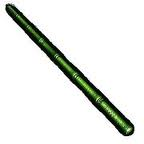
\includegraphics[width=.2\textwidth]{stick}}
    \caption[打狗棒]{\label{fig:stick} 打狗棒}
\end{figure}

\subsection{惡狗攔路}

举棒横在身前,待敌兵器击到,侧抖旁缠,顺势借力向外斜甩,将敌兵器掠在一旁。
\begin{listing}[H]
  \begin{minted}[fontsize=\small,
    linenos=true,numbersep=10pt,
    frame=lines,framesep=10pt,rulecolor=\color{lightgray},
    xleftmargin=4cm, xrightmargin=4cm,
    gobble=4,
    ]{python}
    while true:
        run
  \end{minted}
  \caption{恶狗拦路Python应用示例}
  \label{lst:run}
\end{listing}
恶狗拦路的应用示例如程序~\ref{lst:run}所示。

\subsection{棒打雙犬}
以迅猛之势横扫敌双足。具体应用如程序~\ref{lst:cry}所示。

\begin{listing}[H]
  \begin{minted}[fontsize=\small,
    linenos=true,numbersep=10pt,
    frame=lines,framesep=10pt,rulecolor=\color{lightgray},
    xleftmargin=4cm,xrightmargin=4cm,
    gobble=4,
    ]{c}
    while(dogs == 2){
      cry();
    }
  \end{minted}
  \caption{棒打双犬C应用示例}
  \label{lst:cry}
\end{listing}

\subsection{斜打狗背}
棒身倏地伸出,棒头搭在敌兵器上,轻轻向下按落,以四两拨千斤之理出招。

\subsection{撥狗朝天}
棒身伸出,将敌兵器前端挑甩上来。

\subsection{獒口奪杖}
在竹棒被敌夺去後,伸右手食中二指取敌双目,同时左足翻起,压住棒身,立时夺回,此招变幻莫测,
夺棒时百发百中,纵是武功高已数倍之敌,亦难保全。 

\subsection{棒打狗頭}
以迅猛之势向敌头顶击去。

\subsection{反戳狗臀}
棒身横扫敌臀部。

\subsection{棒挑癩犬}
敌抓住棒身时,前伸斜掠,将棒身挑出。

\subsection{壓扁狗背}
棒身倏地伸出,棒头搭在敌兵器上,轻轻向下按落,以四两拨千斤之理出招。

\subsection{天下無狗}
共有六变,是打狗棒法最后一招最后一变最精妙的绝招,这一招仗将出来,四面八方是棒,劲力所至,
令人难以抵挡,便有几十条恶犬也一齐打死了,所谓“天下无狗”便是此义,棒法之精妙,已臻武学中的
绝诣。

\section{口诀}

\begin{description}
\item[挑字诀:] 棒挑癞犬 歹挑狗身 捣乱狗窝 挑拨狗爪
\item[封字决:] 压扁狗背 饿狗拦路 犬牙交错 母狗护雏   
\item[转字决:] 恶犬回咬 快击狗臀 丧家之犬 黄狗追尾 幼犬戏球   
\item[绊字诀:] 獒口夺杖 拨狗朝天 横打双獒 鸡飞狗跳   
\item[引字诀:] 引狗入寨 棒迥掠地 斜打狗背 摇头摆尾 群狗争食   
\item[戳字诀:] 歹戳狗臀 狗急跳墙 蜀犬吠日 狗眼看人   
\item[缠字诀:] 斗犬十弄 棒打双犬 死拉狗尾 狗咬狗骨 老狗乞怜   
\item[劈字诀:] 棒打狗头 穷巷赶狗 疯狗咬喉 落水打狗 天下无狗
\end{description}

%%% Local Variables: 
%%% mode: latex
%%% TeX-master: "../sample"
%%% End: 

\chapter{一陽指}
一陽指\footnote{参见维基百科 - \href{http://zh.wikipedia.org/wiki/\%E4\%B8\%80\%E9\%99\%BD\%E6\%8C\%87}{《一阳指》}}是金庸武俠小說《射鵰英雄傳》、《神鵰俠侶》與《天龍八部》的一套武功,為雲南大理段氏的獨家武學,擊中時的威力十分巨大。在《射鵰英雄傳》中,「天下五絕」之一的南帝段智興,便是以此武功稱霸天下\cite{yiyangzhi}。

\section{概述}

一陽指為大理段氏的家傳武學,段氏皇族段正明、段正淳、段延慶、段智興皆身具一陽指武功。《射鵰英雄傳》中,曾提及一燈大師段智興已修練到「登峰造極、爐火純青」的境界,並且以一陽指與「天下五絕」之首王重陽交換先天功。一陽指與先天功也是「西毒」歐陽鋒獨門絕學蛤蟆功的剋星。

一陽指有指法以及其獨門的內力,一燈大師曾以多年深厚的一陽指內力替身受重傷的黃蓉治療,但所耗損的內力亦需花多年時間回復,最後一燈幸得《九陰真經》的武功在短時間內恢復。一燈大師將一陽指武功傳給門下弟子「漁樵耕讀」,其中「書生」朱子柳甚至將一陽指與中國書法融合,名為「一陽書指」。《神鵰俠侶》中,「農夫」武三通將一陽指武功分別傳授給兒子武敦儒與武修文,但造詣不深。

《天龍八部》中,大理皇帝段正明與皇太弟段正淳也會使一陽指,「四大惡人」之首段延慶的一陽指造詣亦不遜於
段正明。大理天龍寺中,枯榮大師與門下弟子皆有修練一陽指,其中曾提及鎮寺之寶六脈神劍,便是以一陽指渾厚
的內力化成無形劍氣攻敵,而一陽指在最高第一品時,其境界亦不遜於其他指法武功。

%%% Local Variables: 
%%% mode: latex
%%% TeX-master: "../sample"
%%% End: 

\chapter{双手互搏}
雙手互搏\footnote{参见维基百科 -
  \href{http://zh.wikipedia.org/wiki/\%E5\%8F\%8C\%E6\%89\%8B\%E4\%BA\%92\%E6\%90\%8F}{雙手互
    搏}}(亦稱左右互搏)為金庸武俠小說《射鵰英雄傳》中「老頑童」周伯通\footnote{也就是《神雕俠侶》裡
  的「中頑童」}被「東邪」黃藥師困於桃花島時所創。

\section{概述}
據《神鵰俠侶》\cite{shendiao}原文: 其實這左右互搏之技,關鍵訣竅全在「分心二用」四字。凡是聰明智慧的人,心思繁複, 一件事沒想完,第二件事又湧上心頭。三國時曹子建七步成詩,五代間劉鄖用兵,一步百計,這等人要他學那左右互搏的功夫,便是要殺他的頭也學不會的。

關鍵訣竅全在「分心二用」,因此要習此門功夫,須做到心無雜念。根據周伯通的說法,若能左手畫方,右手畫圓,方能修習此法。《射鵰英雄傳》中世上僅有周伯通、郭靖能使用,《神鵰俠侶》中小龍女以養蜂術與周伯通交換雙手互搏之後便能一人使出「玉女素心劍法」,成為第三個懂得雙手互搏的人。周伯通,郭靖與小龍女皆是心思純樸之人,心無雜念,尤其小龍女自幼便學習寡欲,學習雙手互搏並非難事。

在倚天屠龍記中「崑崙三聖」何足道亦曾以左手凌厲攻敵、右手舒緩撫琴。儘管不及雙手分使兩般武功,卻已是射鵰三部曲中極少數能分心二用的人。

另外,碧血劍中,主角袁承志為圓溫青青一時口舌之快,於擊敗仙都派兩大弟子後,現學現賣,當場使出需兩人才有辦法施展的「兩儀劍法」,書中有云:「只見他雙劍舞了開來,左攻右守,右擊左拒,一招一式,果然與兩儀劍法毫無二致。劍招繁複,變化多端,洞玄和閔子華適才分別使出,人人都已親見,此時見他一人雙劍竟囊括仙都派二大弟子的劍招,盡皆相顧駭然。 」,可見袁承志亦是少數能分心二用之人。

還有《神鵰俠侶》的公孫止的「陰陽倒亂刃法」,能用刀使劍法,劍使刀法,都是一些能分心二用的高手。

%%% Local Variables: 
%%% mode: latex
%%% TeX-master: "../sample"
%%% End: 

\chapter{空明拳}
空明拳\footnote{参见维基百科 - \href{http://zh.wikipedia.org/wiki/\%E7\%A9\%BA\%E6\%98\%8E\%E6\%8B\%B3}{空明拳}}是金庸小說《射鵰英雄傳》、《神鵰俠侶》、《倚天屠龍記》中出現的武功。

空明拳是周伯通被黃藥師困於桃花島時,在所住山洞裡自創的武功。空明拳十六字訣:空朦洞鬆、風通容夢、沖窮中弄、童庸弓蟲。空明拳共七十二路,第一路空碗盛飯、第二路空屋住人、深藏若虛(《神鵰俠侶三六回-獻禮祝壽,耶律齊對上何師我》)、五十四路妙手空空(《倚天屠龍記第一回-天涯思君不可忘,郭襄對上無色》),均為道家的基本概念化成。他在山洞裡和郭靖結為兄弟後,將空明拳傳授給郭靖,之後亦傳給耶律齊。

%%% Local Variables: 
%%% mode: latex
%%% TeX-master: "../sample"
%%% End: 

\chapter{七傷拳}
七傷拳\footnote{参见维基百科 - \href{http://zh.wikipedia.org/wiki/\%E4\%B8\%83\%E5\%82\%B7\%E6\%8B\%B3}{七傷拳}}為金庸武俠小說《倚天屠龍記》中崆峒派的武功,當年崆峒派開山祖師木靈子曾持之威揚天下,但後來崆峒五老內功不足卻強練,因此人人暗伏內傷,反倒從他們手裡奪去秘笈的謝遜更將這門拳法發揮的淋漓盡致,而張無忌則輾轉由謝遜處知悉七傷拳要訣,在維護明教力鬥六大派高手時,在崆峒五老面前炫耀七傷拳功。\footnote{出自倚天屠龍記第二十一章 排難解紛當六強}

\section{介紹}

七傷拳的總訣是四句似歌非歌、似詩非詩的拳訣:「五行之氣調陰陽,損心傷肺摧肝腸,藏離精失意恍惚,三焦齊逆兮魂魄飛揚!」武學宗旨在於先傷己再傷人,一練七傷損及內臟跟陰陽二氣,內力不足者將受創甚深,崆峒五老人人皆練,都暗隱內傷。

由於七傷拳功施展開來威勢顯赫,和成昆的「霹靂拳」等武技外觀類似,但內醞七種迥異拳勁,剛猛、陰柔、剛中有柔、柔中有剛、橫出、直送、內縮兼備。為此謝遜闖入崆峒山青陽觀劫奪拳譜,本來謝遜勢必不敵崆峒五老聯手,但成昆一心挑撥六大派和明教不和,暗地出手相救,用混元功打傷唐文亮、常敬之,使謝遜奪得拳譜,但謝遜馬上著手修練後,傷了心脈導致有時狂性大發\footnote{出自倚天屠龍記第八章 窮發十載泛歸航}。

在謝遜收張無忌為義子後,把七傷拳傳給了張無忌,並在維護明教力鬥崆峒派高手時,張無忌用九陽神功催動七傷拳技壓崆峒五老,但也用九陽真氣暗助宗維俠解除部分內傷,以德服人。由於張無忌的九陽神功極為渾厚,因此他使用七傷拳時完全沒受半點反撲傷害,威力亦更勝崆峒五老跟謝遜。

%%% Local Variables: 
%%% mode: latex
%%% TeX-master: "../sample"
%%% End: 

\chapter{吸星大法}
吸星大法\footnote{参见维基百科 -
  \href{http://zh.wikipedia.org/wiki/\%E5\%90\%B8\%E6\%98\%9F\%E5\%A4\%A7\%E6\%B3\%95}{吸星大法}}是
金庸小說《笑傲江湖》中的一個虛構內功。這套內功是將別人的內力吸收,將這些別人的內力化成自己體內的內力,
或將真氣排出。這吸星大法,創自北宋年間的逍遙派,分為北冥神功與化功大法兩路。後來從大理段氏及星宿派分
別傳落,合而為一,却又偏向化功大法,稱為吸星大法。 

\section{修練難處}

\begin{itemize}
\item 第一,是要散去全身內力,使得丹田中一無所有,只要散得不盡,或行錯了穴道,立時便會走火入魔,輕則全身癱瘓,從此成了廢人,重則經脈逆轉,七孔流血而亡\footnote{取自《笑傲江湖》第二十二章【脫困】}。
\item 第二,散功之後,又須吸取旁人的真氣,貯入自己丹田,再依法驅入奇經八脈以供己用。這一步本來也十分艱難,自己內力已然散盡,再要吸取旁人真氣,豈不是以卵擊石,徒然送命?
\end{itemize}

\section{修練缺陷}

這種內功之中有幾個重大缺陷,初時修練時不會覺,其後禍患卻慢慢顯露出來。如果修練後不理會它,終有一日會
得毒火焚身。那些吸取而來的他人功力,會突然反噬,吸來的功力愈多,反撲之力愈大\footnote{取自《笑傲江湖》
  第二十二章【脫困】}。 

\section{解決方法}

\begin{itemize}
\item 第一,是任我行在梅莊地牢中被困的十二年內發現。書中只提及任我行懂得化解,任我行叫其為融功,但並未提及使用方法。但基本應為使用本身內勁強行壓制。此法雖看似能化解功力反噬之虞,但終究不能長久。
\item 第二,是少林寺方證大師傳授給令狐沖的《易筋經》。在《笑傲江湖》第四十章【曲諧】裡說到,風清揚命方證代傳口訣-「華山內功心法」,但在最後任盈盈對令狐沖說:「沖哥,你到今日還是不明白,你所學的,便是少林派的《易筋經》內功。」
\end{itemize}

%%% Local Variables: 
%%% mode: latex
%%% TeX-master: "../sample"
%%% End: 

\chapter{辟邪劍法}

辟邪劍法\footnote{参见维基百科 - \href{http://zh.wikipedia.org/wiki/\%E8\%BE\%9F\%E9\%82\%AA\%E5\%8A\%8D\%E6\%B3\%95}{辟邪劍法}},金庸武俠小說《笑傲江湖》中的絶世劍法,載有劍法的《辟邪劍譜》,是小說中各人物所爭奪的武林秘笈,亦是引出整個故事的主要書籍\cite{pxjp}。

在令狐沖與少林方证大师、武當沖虛道长密會時,方證與沖虛告訴令狐沖有關劍法的來歷:當年福建少林寺的和尚渡元奉紅葉禪師之命前往華山讨回被華山派门人岳肅與蔡子峰偷錄的《葵花寶典》殘本,但蔡岳二人誤以為渡元禪師曾修習葵花寶典,反而藉機詢問寶典上的武學疑義,渡元一邊以自身武學基礎回應,一邊暗自記憶寶典內容。渡元靠過人記憶力,記下寶典殘本写于袈裟之上,并自創出七十二路《辟邪劍法》,後來也不回福建少林寺,還俗並自稱為林遠圖,開設鏢局,名震江湖。

其後劍譜傳至林震南夫婦時,由於不懂如何練就劍法,因此鏢局之名日墮,並且引來青城派覬覦,掌門人余滄海更將林家滅門以圖奪取劍譜;林家唯一倖存者林平之被華山派掌門岳不群救回並收為弟子。林震南死前向令狐沖留下遺言,使林平之得以尋回劍譜,結果卻落入岳不群手中。岳、林二人靠著劍譜練成驚人武功,最後岳不群與左冷禪在封禪台上決鬥,岳不群以真劍法對抗左冷禪的假劍法,在點瞎左冷禪雙目後取得勝利,成為五嶽派的掌門人,林平之亦得以此劍法報滅門之仇。由於辟邪劍法威名太盛,加上令狐沖得華山派劍宗遺老風清揚傳授獨孤九劍後武功大進,早期亦被岳、林二人懷疑其奪取辟邪劍譜。

與《葵花寶典》的修行方法一樣,練辟邪劍法者必先自宮。而根據曾親眼目睹該劍法的各人所言,劍法本身並無特別厲害之處,全仗自宮後所修練的內功,使劍法威力倍增。而令狐沖與岳不群對戰之時,終領悟到劍法的厲害在於一個「快」字,只要時間一久,劍招便會重複,破綻亦會隨之顯露,令狐沖亦憑此得以破解了辟邪劍法。

%%% Local Variables: 
%%% mode: latex
%%% TeX-master: "../sample"
%%% End: 

\chapter{葵花宝典}
葵花寶典\footnote{\href{http://zh.wikipedia.org/wiki/\%E8\%91\%B5\%E8\%8A\%B1\%E5\%AE\%9D\%E5\%85\%B8}{葵花宝典}},是金庸武俠小說《笑傲江湖》中的禁断的武功秘笈奥義,書中對其來歷著墨不多,相傳作者為前朝\footnote{根據前後文推測前朝为南宋或元朝;金庸言明笑傲江湖不特定某一朝代,根据人物对话及武功推测时间在宋元之后,多数人认为是明朝}
太監,為何太監武功如此高強、卻身居大內,不得而知。此功是以快為主,令人沒有還擊的機會,已將別人打敗\cite{khbd}。

\section{由來}

《葵花寶典》之後流傳到福建少林寺,當時正好華山派门人岳肅與蔡子峰拜訪,趁機各偷抄一部分,被紅葉禪師發覺,認為此害人之物不得留世,於是焚毀。

岳、蔡二人返回華山後,彼此把各自抄寫部分拿出比對,竟然不合,於是互相怀疑以至兄弟反目。

从此二人文爭武鬥,激起華山劍宗與氣宗之爭。小說中風清揚屬劍宗、岳不群屬氣宗。

後日月神教大舉攻入華山派,為的就是奪取《葵花寶典》殘本,激鬥後「日月神教十長老」戰死於華山派,但寶典亦被日月神教奪去,輾轉由東方不敗習得。

上述這一段,乃令狐沖與少林寺方證大師、武當派沖虛道長密會時,由方證與沖虛訴說。

\section{分拆出的武功}

另一段,福建少林寺的和尚渡元奉命前往華山讨要宝典,岳、蔡二人直承不諱,兩人並向渡元禪師請教寶典裡面的武學,認為渡元禪師為紅葉禪師高徒,必有蒙紅葉禪師傳授寶典裡面武學。而渡元靠自身領悟力隨意解釋一番。憑著小部分的記憶,將自己領悟到的記下写于袈裟之上,後來憑此自創出七十二路「辟邪劍法」,後來也不回福建少林寺,還俗並自稱為林遠圖,開設鏢局。該劍谱才是笑傲江湖奪取之主要典籍。

據方證大師所言,林遠圖所悟遠較日月神教奪搶而去之華山派筆錄殘本為多。

\section{修練時的重點}

練習葵花寶典之前,在此典的第一頁已經註明「欲練神功,引刀自宮。煉丹服藥,內外皆通。」(另一說是「欲練此功,必先自宮。不丹不藥,內外皆通」)這句子,意思是修練前必先自宮,否則會『欲火如焚,登時走火入魔,僵癱而死』。東方不敗曾曰:「我初當教主,那可意氣風發了,說什麼文成武德,中興聖教,當真是不要臉的胡吹法螺。直到后來修習《葵花寶典》,才慢慢悟到了人生妙諦。其后勤修內功,數年之后,終于明白了天人化生、萬物滋長的要道。」
另外,岳不群跟林平之都已自宮,但根據金庸原著,岳不群與林平之都不是練《葵花寶典》,因為寶典在日月神教東方不敗之手,兩人練的是由林遠圖改編過的「辟邪劍法」。

\section{其他}

葵花寶典實在的紀載僅一次,亦即在黑木崖上令狐冲、任我行、向問天合攻東方不敗,但僅打成平手,且任我行失去一眼。

在對峙前,東方不敗曾以繡花針攻擊令狐冲,令湖冲以獨孤九劍對應,直擊東方不敗要害的兩敗俱傷打法,逼退東方不敗。東方不敗曾稱讚:「好高的劍法!」

%%% Local Variables: 
%%% mode: latex
%%% TeX-master: "../sample"
%%% End: 

\chapter{九陰真經}
《九陰真經》\footnote{参见维基百科 -
  \href{http://zh.wikipedia.org/wiki/\%E4\%B9\%9D\%E9\%99\%B0\%E7\%9C\%9F\%E7\%B6\%93}{九陰真經}}是
金庸小说中虛構的武學巨著,乃金庸武俠小說系列中最負盛名也最具傳奇性的武學。與《九陽真經》齊名
\cite{jyinzj}。 

\section{傳奇}

\subsection{成書經過}

\subsubsection{初版}
在《射鵰英雄傳》第一版中,《九陰真經》和《九阳真经》原是相傳是達摩祖師所寫下,話說達摩東來,與中土武士較技,雙方互有勝負;面壁九年後參透了武學精奧,寫成二書。
\subsubsection{二版、新修版}
宋徽宗於政和年間,下旨命令一個聰明的刻書人——黃裳刻寫一本道家書籍《萬壽道藏》,共分五千四百八十一卷。由於是為皇帝刻書,黄裳怕出錯殺頭,他花了好幾年小心校對,不知不覺便精通了道學,還領悟了當中的武功。經過慢慢的修練,成了武功高手。

不久,宋徽宗下旨要黄裳派兵去剿滅魔教——明教。不料,當中高手如雲,黄裳遂親自向明教高手挑戰,一口氣殺了
幾個法王使者。哪知道他所殺的人中,有幾個是武林中名門大派的弟子,於是被各大派尋仇,黄裳寡不敵眾,受傷
後逃亡,躲在不毛之地。仇家隨後將他家裡的父母妻兒殺了個乾乾淨淨。為了避免再受追殺,記下了的敵人招式,
苦思破解方法。當他想通了,已經過了四十多年,仇家全都死了。他便覺得自己時日無多,便把畢生心血,寫成上
下两卷的《九陰真經》。

\subsection{重現華山}
天下五絕,即黃藥師、歐陽鋒、段智興、洪七公和王重陽,同意誰勝出誰獨得《九陰真經》。經過七日七夜的大戰,由王重陽奪得。在他臨死前,把《九陰真經》交給周伯通。
\subsection{刻於古墓}
王重陽得知林朝英創出剋制全真教武功的《玉女心經》,不禁佩服起來。後來王重陽奪得《九陰真經》,於是把其中部份武学刻於古墓中,來剋制《玉女心經》。後為楊過、小龍女師徒習得。
\subsection{被人偷竊}
後來,周伯通往桃花島見黃藥師,警告他有人會偷《九陰真經》。黃藥師的妻子馮蘅有機會細閱《九陰真經》的下半部,憑著過目不忘的能力已經把全部內容記下來,再自行書寫出一本交予黃藥師。

不久,黃藥師的徒弟梅超風和陳玄風背叛了黃藥師,偷走了該本《九陰真經》,離開桃花島。黃藥師一怒之下,把所有弟子打跛。身懷六甲的馮蘅為了黃藥師,再度默寫《九陰真經》下卷,但是因為離上次背經已有一段時日,經文已多半忘記了。又因為她努力回想經文導致身心俱疲,生下黃蓉不久就去世了。

另外,陳梅二人離開桃花島後,由於陳梅二人不懂玄門道學,因此陳玄風憑著自己的臆測解經,再轉授梅超風,在
曲解經義的情形下,兩人以「五指插入人的頭蓋骨」或「服用砒霜之毒」等方式,練成了陰毒的「九陰白骨爪」和
「摧心掌」,成了江湖上惡名昭彰的「黑風雙煞」。兩人橫練功夫甚高,不怕擊打,只對利器稍有忌憚。但各自有
個脆弱無比的「罩門」,一碰即死。陳玄風的罩門在肚臍,梅超風的則在舌下。蒙古荒山夜戰中,陳玄風雖以九陰
白骨爪和摧心掌殺了江南七怪的張阿生,卻也被當時年僅六歲的郭靖用匕首刺中罩門而死。梅超風則輾轉到了金國
王府,收楊康為徒,並將九陰白骨爪傳給了楊康。

\subsection{落入郭靖手中}
後周伯通為了作弄郭靖,將九陰真經教給了他,卻不告訴他學的是九陰真經,間接造成黃藥師對郭靖的誤會。
\subsection{藏在倚天劍}
後來郭靖与黃蓉知道襄陽終不可守,將楊過的玄鐵重劍熔了,再加以西方精金,鑄成了一柄屠龍刀,一柄倚天劍,並把《武穆遺書》藏在屠龍刀中,把《九陰真經》與九陰速成之法、《降龍十八掌掌法精要》藏在倚天劍中。 倚天劍被交與女兒郭襄手中,而郭襄則為娥眉派的創始人,後傳承侄滅絕師太,最後落與周芷若手上,屠龍刀下落不明。 多年後於元順帝年間,峨嵋派掌門周芷若放逐汝陽王之女趙敏後,將倚天劍及屠龍刀互砍,取得兵書和武功秘笈而學到九陰白骨爪。其九陰真經內力在身受玄冥神掌之傷後,被張無忌以九陽真經內力醫治時化去大部份。 在新修版中改為兩塊玄鐵鐵片,一為桃花島所在地,一為桃花島地圖,《九陰真經》、《降龍十八掌掌法精義》和《武穆遺書》放在桃花島中心,九陰真經改為完整版。因為金庸感到把書本放到刀劍的夾層中並不合理,鑄造刀劍時會燒去,因此修改為鐵片。
\section{經文選輯}

\begin{itemize}
\item 「天之道,損有餘而補不足,是故虛勝實,不足勝有餘。」
\item 「人徒知枯坐息思為進德之功,殊不知上達之士,圓通定慧,體用雙修,即靜而動,雖攖而寧。」
\end{itemize}

\section{記載神功}

\subsection{上卷(內功)}
\begin{description}
\item[易筋鍛骨篇] 练成后功力等方面均进展迅速。内容提到:「人徒知枯坐息思为进德之功,殊不知上达之士,圆通定慧,体用双修,即动而静,虽撄而宁。」不但有打坐修炼的静功,也有由外而内的动功。
\item[療傷篇] 療傷篇系為療傷之用,亦能用以增加功力。由於能練九陰真經者已有一定修為,故療傷對於一般的外傷亦不多提,主要是談及內傷治方面。
\item[點穴篇] 此篇隻述及點穴方面的要旨,未見有詳細的招式。
\item[解穴秘訣] 为自通穴道之法,可在被人点中穴道或闭塞时,即可用此法自行打通。(《神雕俠侶》第十九回《重陽遺刻》)
\item[移魂大法] 为摄心术的一种,实质有如现代的催眠,能用来对付武功高强,但心志不坚的对手。(君山大會中黃蓉以移魂大法克制彭长老的慑心术)
\item[蛇行狸翻] 即便在地上翻滚,也是灵动异常。(《射鵰英雄傳》第六十二回《阴错阳差》中,周伯通以“蛇行狸翻”避過黃藥師的追擊。)
\item[閉氣秘訣] 运用此法即可长时间不呼吸。(《神雕俠侶》第十九回《重陽遺刻》)
\item[飛絮勁] 《射鵰英雄傳》第三十八回《錦囊密令》中,郭靖以“飞絮劲”化解歐陽鋒一招。
\item[總綱] 此篇為九陰真經的總綱及上卷的最後一章。
以梵文譯音寫成,初版作者為達摩,自無問題,二版卻成為黃裳為免九陰真經落入歹人之手而加防備的一種手段。九陰真經總綱精奧無比,能將修真之士所遇的幻象之類,轉為神通。
新版九陰真經總綱更糾正了道家武學偏重陰柔的流弊,實現了陰陽互濟、剛柔並重的武學最高境界。  
\end{description}
\subsection{下卷(武功)}
\begin{description}
\item[摧心掌] 中此掌者,外在并无任何伤痕,但内裡的五脏六腑已然碎裂。
\item[白蟒鞭法] 使用極長的白蟒鞭,如靈蛇出洞,伸縮自如,靈動之極。
\item[大伏魔拳] 稳实刚猛之气的掌法,招数神妙无方,拳力笼罩之下威不可挡。 (《神鵰俠侶》中,周伯通以大伏魔拳與楊過的「黯然銷魂掌」對拆)
\item[收筋縮骨法] 君山大會中郭靖以此“收筋缩骨法”脫縛。(《射雕英雄傳》第二七回\cite{shediao})
\item[摧堅神爪] 五指发劲,无坚不破,摧敌首脑,如穿腐土,出爪时爪心有强大的吸力可隔空取物或吸取他人功力,爪指有强大的透劲可隔空伤人,一收一放,一开一合,合乎武学大道之理。
\item[九阴白骨爪] 受此功夫死亡者头顶五个指洞,是极为阴险的工夫,但其实为一正而不邪的功夫,九阴白骨爪
  在《九阴真经》中原是“摧堅神爪”,「铜尸」陈玄风、「铁尸」梅超风学不到《九阴真经》上半部中养气归元、
  修习内功的心法,但凭已意,胡乱揣摸,不知“摧敌首脑”是「攻敌要害」之意,以为是以五指去插入敌人头盖,
  又以为练功时必须如此,硬是把上乘武功练到了邪路上。和峨眉派掌门周芷若都为求速成,亦练得此功,夺得武
  功天下第一的名头。

  註:二版中,九陰白骨爪為黑風雙煞錯練九陰神爪而成,真經中本無白骨爪;新三版增寫九陰白骨爪等功為黃裳
  之敵的武功,黃裳弟妹便死於此功之手,黃裳便創摧堅神爪以破白骨爪。另二版中本無白蟒鞭法,只有梅超風的
  兵器毒龍鞭及真經中一套無名鞭法;新三版中毒龍鞭易名白蟒鞭,並加上白蟒鞭法。 
\end{description}

%%% Local Variables: 
%%% mode: latex
%%% TeX-master: "../sample"
%%% End: 

\chapter{九陽真經}
《九陽真經》\footnote{参见维基百科 - \href{http://zh.wikipedia.org/wiki/\%E4\%B9\%9D\%E9\%99\%BD\%E7\%9C\%9F\%E7\%B6\%93}{九陽真經}}是金庸小說中虛構的武學巨著\cite{jyangzj}。

《九陽真經》是這本內功秘集的名稱。內功練成,便名《九陽神功》,乃是金庸武俠小說系列中極強、甚至最強的內功,被喻為非任何內功所能比。與《九陰真經》齊名。

金庸武俠小說系列中練成全套《九陽神功》的人物,除了創者,就只有《神鵰俠侶》、《倚天屠龍記》中的僧人覺
遠,以及《倚天屠龍記》的主角張無忌練成。

\section{成書經過}
在《倚天屠龍記》第一版中,《九陽真經》與《九陰真經》相輔相成,同是達摩所寫下。《九陰真經》有無數神妙武功,《九陽真經》雖然只有內功,但神功大成後,卻非世上的任何武功所能傷害。

二版中,《九陰真經》變成黃裳所創,《九陽真經》則是相傳是達摩祖師所寫下的,但後來張君寶悟到達摩祖師是天竺人,就算會寫中華文字,也必文理粗疏,九陽真經文字佳妙,外國人決計寫不出,定是後世中土人士所作。多半便是少林寺中的僧侶,假托達摩祖師之名,寫在天竺文字的《楞伽經》夾縫之中。

在最新修改版本中,作者寫成在嵩山中一位奇士鬥酒勝了王重陽,得以借觀《九陰真經》,此人觀看後覺得《九陰真經》陰氣太重,一味崇揚老子之學,只重以柔克剛,以陰勝陽,未及陰陽互濟之妙,於是在四卷梵文《楞伽經》的行縫之中,寫下自創的《九陽真經》。

然而,新修版《射鵰英雄傳》的《九陰真經》總綱卻明言「九陰極盛」乃是災害,總綱的要旨亦是要糾正這一毛病,故此奇士所見,應不包括《九陰真經》的梵文總綱。《九陰真經》的梵文總綱與九陽真經相同,皆為「陰陽互濟」之道。若修習成功,便與九陽真經達到相同的「武學最高境界」。
\section{重見天日}
於《神鵰俠侶》中,楊過打敗金輪法王(新修版改稱「金輪國師」)後,蒙古武士尹克西和瀟湘子逃到嵩山,後發
現張君寶(後來的張三丰)在少林寺廊下讀《楞伽經》,尹克西悄悄走到他身後,伸手點了他的穴道,把那四卷
《楞伽經》取去。


\section{經在猴中}
後來,張君寶的師父覺遠追尹克西和瀟湘子到華山,巧遇楊過、小龍女和郭襄。尹克西和瀟湘子眼看無法脫身,剛
好身邊有只蒼猿,兩人心生一計,便割開蒼猿肚腹,將經書藏在其中。後來覺遠、張君寶、楊過等搜索瀟湘子、尹
克西二人身畔,不見經書,便放他們帶同蒼猿下山。後來瀟湘子和尹克西帶同蒼猿,遠赴西域,兩人心中各有所忌,
生怕對方先習成經中武功,害死自己,互相牽制,遲遲不敢取出猿腹中的經書,最後來到崑崙山的驚神峰上,尹湘
兩人互施暗算,鬥了個兩敗俱傷而死。這部修習內功的無上心法,從此留在蒼猿腹中。

\section{覺遠傳經}

尹克西臨死時遇見「崑崙三聖」何足道,良心不安,請他赴少林寺告知覺遠大師,那部經書是在這頭蒼猿的腹中。但他說話之時神智迷糊,口齒不清,他說「經在猿中」,何足道卻聽做「金在油中」。何足道信守然諾,果然遠赴中原,將這句「金在油中」的話跟覺遠說了。覺遠無法領會其中之意,固不待言,反而惹起一場絕大的風波,令覺遠、張君寶被少林寺所逐。覺遠圓寂前,念起《九陽真經》,令郭襄、張君寶和少林寺羅漢堂首座無色禪師各有所悟,無色得其高(因三人中武功最高並與其本身武功印證),郭襄得其博(因家學淵博,所學甚廣),張君寶得傳承最多,後來郭襄、張君寶出家開創峨嵋、武當,各以此為基礎,創出了少林九陽功、峨嵋九陽功、武當九陽功,共三脈《九陽功》。

後來《倚天屠龍記》中張無忌因朱子柳的後代朱長齡的掀連意外地進入崑崙山一山谷,巧遇當年的蒼猿,因好心治
療的其肚腹上的傷痕,取出內藏之經書,得以習得完整的九陽神功,不但纏綿體內的寒毒盡皆驅除,內力更提升至
絕高的境界。待得到乾坤一氣袋的奇遇後,張無忌的九陽神功方克大成。

\section{永埋土中}
在張無忌走進崑崙山山谷後五年,他學全了九陽真經,於是把四卷載有《九陽真經》的《楞伽經》、以及胡青牛的
《醫經》、王難姑的《毒經》埋在地洞裡。

\section{經文選輯}
\begin{itemize}
\item 「他強任他強,清風拂山崗;他橫任他橫,明月照大江。」
\item 「他自狠來他自惡,我自一口真氣足。」
\end{itemize}

\section{龍虎門的九陽神功}

在龍虎門,主角王小虎依此絕學而踏入頂級高手的領域,而白蓮教教主東方無敵的九陽神功乃是練的最出神入化的
一個。自古以來,江湖傳言「九陽神功驚俗世」,「君臨天下易筋經」,這兩套絕學號稱頂級絕學。然而,東方無
敵武學智慧卻突破原有九陽神功的範疇,成就九陽五絕合一。武學領域已達至前無古人的十陽聖火,媲美黑級高階
功力甚至超越黑級高階。白蓮教是東方家族企業,由於無懼未指派繼承人就駕崩,故無忌及無敵以武論尊,最終無
敵擊敗無忌就任白蓮教主,所以東方無敵與火雲邪神及文珠天尊不同的地方就在於他必須靠自己的努力,沒有其他
人可依靠,羅剎教的第二號人物是老邪神,通天教的第二號人物則是文珠天尊自己,因為第一號人物是老天尊,白
蓮教就缺乏與他們並駕齊驅的強者。雄才大略的東方無敵向羅剎教挖角金羅漢成為日聖使,同時也向龍虎門挖角王
風雷擔任月聖使,這新的鐵三角,遠比之前日月聖使還強,甚至在《王風雷傳》中號稱「無敵組合」,而《新著龍
虎門》中,白蓮教也相當聰明,不跟強橫的龍虎門為敵。

龍虎門的九陽神功分內功和外功\footnote{(按:此處非金庸小說,乃他書中雷同之武學名稱。)}。

\subsection{內功:九陽真經}

\begin{description}
\item[九陽神功之十陽聖火:]九陽神功第十陽突破原有九陽神功的範疇,媲美黑級高階功力甚至超越黑級高階。
\item[九陽神功之九陽合一:]東方無敵在黑龍就任羅剎教主的登位大典上使用的「九陽合一」,所發出的「九陽
  大霹靂」威力強橫,三皇全力發出「九陰大霹靂」也只能拼成平手,而這個戰績已經媲美神山之役時火雲邪神的
  易筋經黑級高階功力。這些是不是就說明「九陽合一」被設定為媲美黑級高階功力呢? 
\item[九陽神功之九陽歸一:]發揮九陽的顛峰境界,可令神功進入另一層次。
\item[九陽神功之九陽啟泰:]號稱九陽神功頂級功力。
  \begin{multicols}{2}
    \begin{enumerate}
    \item 第九陽百會穴
    \item 第八陽至陽穴
    \item 第七陽脊樑穴
    \item 第六陽手少陽三焦經穴
    \item 第五陽手太陽小腸經穴
    \item 第四陽足太陽膀胱經穴
    \item 第三陽足陽明胃經穴
    \item 第二陽丹田穴
    \item 第一陽心坎穴
    \end{enumerate}
  \end{multicols}
\end{description}

\subsection{外功:九陽五絕}

\begin{description}
\item[第一絕:]霹靂神掌[九陽霹靂]:九陽五絕中威力最強最驚世駭俗的掌法。只有降龍掌可與之一拚。 
  \begin{enumerate}
  \item 九陽小霹靂:練到九陽是可以控制方向的,練到八陽就只能當普通的直線型氣功炮。
  \item 九陽大霹靂:彷彿超巨能靈彈,威力無堅不摧,「火雲邪神」曾敗於此招下。
  \item 雙霹靂合璧:風雷傳裡凶星助無敵升級,無敵打出的霹靂威力可能接近雙陽霹靂合璧的威力,這招號稱天
    上無人能擋。
  \end{enumerate}
\item[第二絕:]九陽神劍:用手指發出劍氣傷敵;最強招「雙陽劍合璧」,需第八陽以上功力方可使用。
  \begin{multicols}{3}
    \begin{enumerate}
    \item 大商劍
    \item 少商劍
    \item 大衝劍
    \item 少衝劍
    \item 大澤劍
    \item 少澤劍
    \item 大陽劍
    \item 少陽劍
    \item 雙陽劍
    \end{enumerate}
  \end{multicols}
\item[第三絕:]陰陽大挪移:可卸開敵人招式,有外傷時不可使用,否則血流不止。
\item[第四絕:]火雲掌:掌法絕學。白蓮教死對頭羅剎教教主學得此掌法,故號稱「火雲邪神」以羞辱白蓮教。[來源請求]
  \begin{multicols}{3}
    \begin{enumerate}
    \item 火雲鐵桶
    \item 火蛇吐信
    \item 火龍穿山
    \item 火雲蓋頂
    \item 火海無邊
    \item 地火燎原
    \item 天火焚城
    \end{enumerate}
  \end{multicols}
\item[第五絕:]烈陽刀:以掌為刀,招法剛猛
  \begin{multicols}{2}
    \begin{enumerate}
    \item 第一式:烈陽普照
    \item 第二式:烈陽雙暉
    \item 第三式:烈陽破頂
    \item 第四式:烈陽焦土
    \item 第五式:烈陽焚天
    \end{enumerate}
  \end{multicols}
\item[五絕合一:]東方無忌 (王風雷傳十二期對東方無忌使用的連續技,並在三十九期命名)
\end{description}


%%% Local Variables: 
%%% mode: latex
%%% TeX-master: "../sample"
%%% End: 

\chapter{全真剑法}
全真劍法
\footnote{参见维基百科 - \href{http://zh.wikipedia.org/wiki/\%E5\%85\%A8\%E7\%9C\%9F\%E5\%89\%91\%E6\%B3\%95}{全真劍法}}是全真教的基礎劍法。华山派剑法即为其残缺补全版,峨嵋派剑法中也有直接借用全真剑法的招数。古
墓派亦有一套玉女劍法專克全真劍法,但當雙劍合壁,一個使玉女劍法,一個使全真劍法,就會變成威力極大的玉
女素心劍法。

%%% Local Variables: 
%%% mode: latex
%%% TeX-master: "../sample"
%%% End: 

\chapter{摧心掌}
摧心掌\footnote{参见维基百科 - \href{http://zh.wikipedia.org/wiki/\%E6\%91\%A7\%E5\%BF\%83\%E6\%8E\%8C\_(\%E4\%B9\%9D\%E9\%99\%B0\%E7\%9C\%9F\%E7\%B6\%93)}{摧心掌}}是金庸小說《射鵰英雄傳》中的一門十分殘酷和利害的掌法。

\section{簡介}

此掌雖名「摧心」,但中者五臟六腑皆會被震爛,骨骼卻不折斷。《射鵰英雄傳》中,「銅屍」陳玄風、「鐵屍」梅超風夫妻偷取師父黃藥師的《九陰真經》,練就經上九陰白骨爪、白蟒鞭法、橫練功夫外以及此功。但因黑風雙煞夫妻多用白骨爪及白蟒鞭法而少用摧心掌,摧心掌的知名度遠遜上述二功。

後來,銅屍鐵屍先後伏誅,九陰真經正本被毀,郭靖夫妻、楊過夫妻亦未曾練就此功,相信摧心掌就此失傳。

然而笑傲江湖中青城派掌門余滄海亦會同名而相似的武功。


%%% Local Variables: 
%%% mode: latex
%%% TeX-master: "../sample"
%%% End: 

\chapter{降龍十八掌}
降龍十八掌\footnote{参见维基百科 - \href{http://zh.wikipedia.org/wiki/\%E9\%99\%8D\%E9\%BE\%8D\%E5\%8D\%81\%E5\%85\%AB\%E6\%8E\%8C}{降龍十八掌}}是金庸武俠小說《天龍八部》、《射鵰英雄傳》、《神雕侠侣》\cite{shendiao}和《倚天屠龍記》\cite{yitian}中丐幫二大謢幫神功之一,降龍十八掌分為十八式。

世紀新修版的《天龍八部》中,則改為降龍廿八掌,對應天上二十八星宿,後來才由乔峰及虛竹簡化為十八掌。

\section{簡介}
降龍十八掌講究剛柔並濟,當剛則剛,當柔則柔,轻重刚柔随心所欲,刚劲柔劲混而为一,劲力忽强忽弱,忽吞忽吐,从至刚之中生出至柔,天下阳刚第一,掌法之妙,天下无双,招招须用真力,说是外门武学中的巅峰绝诣,動作雖似簡單無奇,但掌掌現神龍,招招威力無窮,招式简明而劲力精深的武功,精要之处,全在运劲发力,全凭劲强力猛取胜,当真是无坚不摧、无固不破,虽招数有限,但每出一掌均有龍吟虎嘯之勢、每出一招均具绝大的威力。

降龍十八掌原為廿八掌,從創幫之主傳承自汪劍通再傳到蕭峰時,因為後十招過於繁瑣,且威力卻遠不如前十八掌,經虛竹和蕭峰刪除重複後,威力更勝一籌,在蕭峰死後由虛竹把降龍十八掌代傳下任幫主,又輾轉授至洪七公之手。

由於降龍十八掌並非只傳幫主繼承人,所以洪七公也教給了郭靖和立有大功的黎生一招「神龍擺尾」,甚至郭靖也曾傳授給武敦儒、武修文兄弟,在第一版的倚天屠龍記中武家後人武烈也有降龍十八掌的部分秘笈,謝遜也曾教給張無忌些許降龍十八掌的招式,但是在後來的改版中這些內容都刪去。當郭靖女婿耶律齊接任丐幫幫主後,郭靖亦授他降龍十八掌,但因為襄陽被攻陷時,郭家眾人多殉國身亡,耶律齊後任的幫主並沒學全,只練成其中十四掌,後來傳到史火龍時只剩十二掌,在他被成昆殺害後,這門掌法似乎便告失傳,笑傲江湖時代的解風明顯不會這門掌法。

降龍十八掌的大部分招式的名字由易經而來,包括:
\begin{enumerate}
\item 亢龍有悔(乾卦上九): 其招式为左腿微屈,右臂内弯,右掌划一圆圈,向外推去。
\item 飛龍在天(乾卦九五): 这一招必先跃起半空,居高下击,才能显见奇大的威力,它一定要配合轻功跳跃之技,由上而下给予敌人痛击,算起应该是一种技巧性较高的武技。
\item 龍戰於野(坤卦上六): 左臂右掌,均是可虚可实,非拘一格。用虚实相生,阴阳相参的手法扰乱对方,自己则可以趁虚而入,是一式诱敌策。
\item 潛龍勿用(乾卦初九): 则是右手屈起食中二指,半拳半掌,向敌人胸口打去,左手同时向里钩拿,右推左钩,让敌人难以闪避。这是一种左右夹击的攻势,让人无处可避,尽在自己的掌握之中。
\item 利涉大川(大畜、同人、未济等卦多次出现): 逼退敌人之招式,用意在于使敌人勿近其身,以为自保。
\item 鴻漸於陸(漸卦九三): 此两招是一种技术性的逼退敌人之招式,用意在于使敌人勿近其身,以为自保。
\item 突如其來(離卦九四)
\item 震驚百里(震卦彖辭): 双掌向前平推,这是降龙十八掌中威力极大的一招。
\item 或躍在淵(乾卦九四): 先提一口气,然后以气化掌,左掌前探,右掌嗖的从左掌下穿了出去,直击对手小腹。是属于一种至刚至阳的正面攻势。
\item 神龍擺尾(原名履虎尾,履卦九四): 此乃降龙十八掌救命绝招,任何有生命的东西在他有生存受到威胁时所生成而出的反应力道,自是非同小可。
\item 見龍在田: 这一招是用于狭小空间的防身之术,它或为缓冲高手绵密不绝的攻势之用。
\item 雙龍取水(乾卦彖辭): 这一招转守为攻之策,当手腕被别人擒拿,此招可以顺腕翻过,以又重又快的掌法拍击敌人肩头,是一招转守为攻的法门。
\item 魚躍於淵(小畜卦辞): 此招由下而上的攻敌之术,与飞龙在天相为反生,是一种败中求胜之道。
\item 時乘六龍(乾卦九二)
\item 密雲不雨(損卦彖辭)
\item 損則有孚(坤卦初六)
\item 履霜冰至(大壯上六): 肘往上微抬,右拳左掌,直击横推,一快一慢的打出去。掌法之中刚柔并济,正反相成,实是妙用无穷,为“降龙十八掌”中较为阴柔的一技。
\item 羝羊觸藩(震卦初九): 意欲以掌力内功和着全身的体重,以快速的步伐,让敌人避无可避射无可射,其姿态就如一只受到刺激的羊一样,不顾一切地想冲出栅栏,威力相当惊人。
\end{enumerate}

\section{出入}
該武功在金庸小說中有出入。在《射鵰英雄傳》初版中,洪七公曾說這些有一半是自創的,但是在《天龍八部》中,丐幫幫主喬峰學會了全部十八式,且至死都未收徒授藝,前後矛盾。後來在第三版時才修正成洪七公僅為傳承者,並無自創招式。\footnote{順帶一提的是,丐幫之寶打狗棒也在喬峰任上遺失,但後來洪七公卻手持打狗棒,甚至與「西毒」歐陽鋒對戰,最後還傳給黃蓉。此漏洞亦於第三版時修正。}
\section{改編自降龍十八掌的武功}
由於金庸所創造武功「降龍十八掌」之名氣甚大,因此在之後出現了許多參考或托名「降龍十八掌」的武功。
\subsection{武狀元蘇乞兒}
降龍十八掌亦在周星馳主演的電影《武狀元蘇乞兒》中出現,與金庸小說的版本相似,這門武功同屬於丐幫幫主相傳的。

\begin{multicols}{3}
  \begin{enumerate}
  \item 飛龍在天
  \item 神龍擺尾
  \item 黑龍偷心
  \item 雙龍出海
  \item 見龍在田
  \item 龍飛鳳舞
  \item 伏虎降龍
  \item 縮龍成寸
  \item 龍蛇混雜
  \item 龍的傳人\footnote{是周星馳其他電影的名稱}
  \item 龍鳳呈祥
  \item 龍馬精神
  \item 望夫成龍\footnote{是周星馳其他電影的名稱}
  \item 殺龍有悔
  \end{enumerate}
\end{multicols}
%%% Local Variables: 
%%% mode: latex
%%% TeX-master: "../sample"
%%% End: 

\chapter{六脈神劍}
六脈神劍
\footnote{参见维基百科 -
  \href{http://zh.wikipedia.org/wiki/\%E5\%85\%AD\%E8\%84\%88\%E7\%A5\%9E\%E5\%8A\%8D}{六脈神劍}}是
金庸武俠小說中的一套武功,使用者為《天龙八部》主角之一—段譽,堪稱大理段氏最厲害的武功, 讓段譽面對敵
手時幾乎所向無敵,但因段譽對武功的瞭解不夠透徹,實戰經驗也不足,常面臨時靈時不靈的情況, 威力也有所折扣。

\section{簡介}
六脈神劍,並非真劍,乃以渾厚內力的指力發出六種內力,含於指尖的內力隔空激發出去,使其以極高速在空中運動的一門技術,做架簡單,功效卓著,感應強烈,均為首屈一指,久習可得奇效。達到指劍的境界,即指力所能及的地方,有如有一柄無形的劍,無論是橫掃或虛指,均可傷敵,劍氣有質無形,出劍時急如電閃,迅猛絕倫,交叉運用,以氣走劍殺人於無形,異常神奇,堪稱劍中無敵,可稱無形氣劍。

它為大理段氏天龍寺鎮寺之寶,不傳段氏俗家子弟,只有天龍寺僧人,方蒙傳授。六脈神劍源自於人體中十二經脈
中的六脈—手太陰肺經、手陽明大腸經、手少陰心經、手少陽三焦經、手厥陰心包經、手太陽小腸經。

\section{六脈運行}

\subsection{右手剑}
\begin{itemize}
\item 右手拇指─少商劍〈特點:劍路雄勁,頗有石破天驚,風雨大至之勢〉:
中府→天府→尺澤→孔最→列缺→經渠→太淵→魚際→少商,屬於「手太陰肺經」。
\item 右手中指─中衝劍〈特點:大開大闔,氣勢雄邁〉:
天池→天泉→曲澤→郄門→間使→大凌→勞宮→中衝,屬於「手厥陰心包經」。
\item 右手小指─少衝劍〈特點:輕靈迅速〉:
極泉→青靈→少海→靈道→通里→陰郩→神門→少府→少衝,屬於「手少陰心經」。
\end{itemize}
\subsection{左手剑}
\begin{itemize}
\item 左手食指─商陽劍〈特點:巧妙靈活,難以捉摸〉:
迎香→扶突→天鼎→肩與→曲池→手三里→陽溪→合谷→商陽,屬於「手陽明大腸經」。
\item 左手無名指─關衝劍〈特點:以拙滯古樸取勝〉:
絲竹空→耳門→翳風→肩髎→天井→支溝→外關→陽池→中渚→液門→關衝,屬於「手少陽三焦經」。
\item 左手小指─少澤劍〈特點:忽來忽去,變化精微〉:
聽宮→顴髎→天容→天窗→肩中俞→秉風→天宗→臑俞→小海→支正→養老→腕骨→后谿→少澤,屬於「手太陽小腸經」。
\end{itemize}

\section{六脈神劍經}
大理天龍寺的鎮寺之寶,大理國祖師爺段思平所創,大理段氏的至高無上武功。

故老相傳,其與易筋經為武林兩大不世瑰寶,經上記載六脈神劍的修鍊方法,總共有六張圖譜,每幅圖上的劍氣圖都是縱橫交叉的直線、圓圈和弧形。

由於六脈神劍不傳段氏俗家子弟,所以連段正淳等人也不知曉《六脈神劍經》藏於天龍寺。

在吐蕃國師鳩摩智強行取經的事件中,枯榮為了不讓經書落入外人手中,以「一陽指」內力將圖譜焚毀。

由於枯榮等六人各學得一路劍法,段譽也將六式劍招全學齊,讓六脈神劍不致失傳。

%%% Local Variables: 
%%% mode: latex
%%% TeX-master: "../sample"
%%% End: 

\chapter{兰花拂穴手}
兰花拂穴手\footnote{参见百度百科 - \href{http://baike.baidu.com/view/1222399.htm?func=retitle\#sub1222399}{兰花拂穴手}},那是黄蓉的独门武功。书中记载,拇指与食指扣起,余下三指略张,手指如一枝兰花般伸出,姿势美
妙已极。讲究“快、准、奇、清”。尤以”清”字诀最难,需出手优雅,气度闲逸,轻描淡写,行若无事。

\section{简介}
兰花拂穴手,那是黄蓉的独门武功。书中记载,拇指与食指扣起,余下三指略张,手指如一枝兰花般伸出,姿势美
妙已极。讲究“快、准、奇、清”。尤以”清”字诀最难,需出手优雅,气度闲逸,轻描淡写,行若无事。

\section{招式}
拇指与食指扣起,余下三指略张,手指如一枝兰花般伸出,姿势美妙已极。讲究 “快、准、奇、清” 。尤以”清”字
诀最难,需出手优雅,气度闲逸,轻描淡写,行若无事。亦可与落英神剑掌合用,指化为掌,掌化为指,掌来时如
落英缤纷,拂指处若春兰葳蕤,不但招招凌厉,而且丰姿端丽。

\section{八大基本按摩手法}
就芳香按摩而言,手法都是较轻柔的,因为轻柔兰花拂穴手的手法才能唤醒最细微的感知细胞,也才能使身心更健康。

芳香按摩的手法其实可以自行变化,只要你能掌握这四点原则:
\begin{enumerate}
\item 用心按摩,让受按摩者感到温暖。
\item 动作缓慢,不可过於急躁使受按摩者更紧张。可随时询问被按摩者的感受,以调整按摩的力道。
\item 配合受按摩者的呼吸进行按摩手法,会使过程更顺畅、按摩者感觉更舒服。
\item 带著觉知进行。以传达关爱、温暖的心情进行按摩,受按摩者会有完全不一样的感受,这虽然是很细微、无
  法言喻的,但却真的能用心感受得到。 
\end{enumerate}
为桃花岛功夫,黄药师与黄蓉父女俩会用(见金庸《射雕英雄传》)。

黄蓉在给郭靖和洪七公做菜时曾在做豆腐时用了兰花拂穴手,使洪七公赞不绝口(见金庸《射雕英雄传》。

%%% Local Variables: 
%%% mode: latex
%%% TeX-master: "../sample"
%%% End: 

\chapter{落英神剑掌}
落英神剑掌\footnote{参见百度百科 - \href{http://baike.baidu.com/view/84720.htm\#sub84720}{落英神剑掌}}又名桃华落英掌,武侠小说中的武功,这套掌法的名称中有“神剑”二字,是黄药师从剑法中变法而得。
出掌凌厉如剑,招数繁复奇幻。双臂挥动,四面八方都是掌影,或五虚一实,或八虚一实,真如桃林中狂风忽起,
万花齐落一般。虚招固为诱敌扰敌,但到临阵之时,五虚八虚亦均可变为实招。

\section{简介}
落英神剑掌又名桃华落英掌,武侠小说中的武功,这套掌法的名称中有“神剑”二字,是黄药师从剑法中变法而得。
出掌凌厉如剑,招数繁复奇幻。双臂挥动,四面八方都是掌影,或五虚一实,或八虚一实,真如桃林中狂风忽起,
万花齐落一般。虚招固为诱敌扰敌,但到临阵之时,五虚八虚亦均可变为实招。黄药师被全真七子天罡北斗阵所围
时,便曾以此掌法酣斗七子(见金庸《射雕英雄传》)。

\section{特点}
落英神剑掌为一奇妙武学,被写在桃花岛主竹亭之上:“桃花影里飞神剑。”足见药师为此之自负。只见黄蓉使来,
虚实变化繁复,拳掌翻飞,潇洒有余,却不及降龙十八掌之刚正威猛,玉萧剑法 桃花岛绝学,有飘逸出尘之姿。

\section{记载}
此掌法黄蓉曾经在洪七公面前与郭靖比武时用过,结果被洪七公发现,虽然此掌法不被其他人所知,但是洪七公从
武功路数上看出是桃花岛的武功。

桃花岛主黄药师的落英神剑掌法,是集其毕生心血所创的绝世掌法,身法奇异、恣意脱俗,江湖上想一窥面貌的不
知凡几;但桃花岛上机关重重,想要闯过这五行八卦之阵都万分困难了,更遑论是想一睹这落英神剑掌的精妙了。
但武林近日盛传黄药师出现在中原地区的消息,这也许会是一个与其结交的大好机会!

%%% Local Variables: 
%%% mode: latex
%%% TeX-master: "../sample"
%%% End: 

\chapter{碧海潮生曲}
《碧海潮生曲》\footnote{参见维基百科 - \href{http://zh.wikipedia.org/wiki/\%E7\%A2\%A7\%E6\%B5\%B7\%E6\%BD\%AE\%E7\%94\%9F\%E6\%9B\%B2}{《碧海潮生曲》}}最初是金庸武俠小說中黃藥師所創的武功乐曲。

東邪黃藥師精通琴、棋、書、畫、醫、卜、兵、陣,他自創的這首《碧海潮生曲》,表面上簫聲聽似模仿大海潮浪之聲,其實內藏極高度致命武功,聲情致飄忽,纏綿宛轉,若在無防備之下聆聽則難以自制,不住手舞足蹈,甚至胡亂抓搔頭臉。


台灣作曲家劉學軒以《碧海潮生曲》為主題,使用曲笛與古箏首度將此乐曲搬上舞台。首演時間為2006年9月16日,地
點為台灣國家演奏廳,於國家國樂團「笑傲江湖」音樂會中世界首演。

%%% Local Variables: 
%%% mode: latex
%%% TeX-master: "../sample"
%%% End: 

\chapter{龍爪擒拿手}
龍爪擒拿手
\footnote{参见维基百科 - \href{http://zh.wikipedia.org/wiki/\%E9\%BE\%8D\%E7\%88\%AA\%E6\%93\%92\%E6\%8B\%BF\%E6\%89\%8B}{
    龍爪擒拿手}}為金庸武俠小說《倚天屠龍記》中之武功,乃少林七十二絕技之一,是空性在光明頂激戰張無忌
時所用的武功。

\section{簡介}

龍爪擒拿手是少林七十二絕技之一,乃少林派四大神僧中空性的絕技,雖說四大神僧全都練就,但以空性造詣最高。

龍爪手全套只有三十六招,要旨端在凌厲狠辣,不求變化繁多。空性中年之時曾數逢大敵,僅要使出龍爪手便立占上風,通常用到十二招便即取勝,從第十三招起,只是空性自己平時練習之用。

被張無忌評說是沒有破綻的不敗武功,藉由身法拉開兩、三尺距離後,仔細端詳偷學模仿,最後用一模一樣的龍爪手破解空性的龍爪手,兩人英雄識英雄反倒結交。

在少林派離開光明頂後,空性一路被蒙古軍伏撃時,因提早發現對方使用時香軟筋散暗算而起衝突,空性以「龍爪
擒拿手」與汝陽王府旗下西域少林金剛門僧人「阿三」的「大力金剛指」大戰時,指力鬥指力,空性不敵被殺\footnote{出自倚天屠龍記第二十四章 太极初傳柔克剛}。

\section{招式}

書中有記載的招式,記載如下\footnote{出自倚天屠龍記第二十一章 排難解紛當六強}:

\begin{itemize}
\item 第八招「拿雲式」:左手虛探,右手挾著一股勁風,直拿人左肩缺盆穴。
\item 第十二招「搶珠式」:此招和拿雲式外表雖同,但方位卻異,雙手一樣自上而下同抓,卻是抓人左右太陽穴。
\item 第十七招「撈月式」:虛拿人後腦風府穴。
\item 捕風式、捉影式、撫琴式、鼓瑟式、批亢式、擣虛式:套路不明,八式連環不絕,便如一招中的八個變化一般,快捷無比。
\item 第三十五招「抱殘式」、第三十六招「守缺式」:龍爪手最後兩招,至剛生柔,看似破綻百出,實則暗藏陷阱。
\end{itemize}

%%% Local Variables: 
%%% mode: latex
%%% TeX-master: "../sample"
%%% End: 

\chapter{火焰刀}
火焰刀\footnote{参见维基百科 - \href{http://zh.wikipedia.org/wiki/\%E7\%81\%AB\%E7\%84\%B0\%E5\%88\%80}{火焰刀}}為
金庸武俠小說《天龍八部》中之武功,乃密教寧瑪派的神奇武功,可將虛無縹緲的掌氣凝刀刃之利,不可捉摸,能
殺人于無形\footnote{出自天龍八部第十章 劍气碧煙橫}。

\section{介紹}

火焰刀是鳩摩智在吐蕃密教寧瑪派出家,因與吐蕃國黑教邪徒鬥爭劇烈,從寧瑪派上師處學得之武技,能以內力凝聚於手掌掌緣,運氣送出劈砍敵手,所以雖屬掌法卻以刀為名。鳩摩智曾憑藉這門武功和天龍寺的六脈神劍陣劇鬥一場,後來也曾多次用於應敵。

在金庸進行修改後的新三版中,鳩摩智能從慕容博手裡獲得少林七十二絕技,就是用火焰刀的修練法訣交換,也被慕容博評說火焰刀動念即發,猶勝發勁緩慢的一陽指,並提及和火焰刀有相同妙用但可發發六種內力的六脈神劍,引起鳩摩智日後往天龍寺奪經的遠因。

%%% Local Variables: 
%%% mode: latex
%%% TeX-master: "../sample"
%%% End: 

\chapter{黯然銷魂掌}
黯然銷魂掌
\footnote{参见维基百科 - \href{http://zh.wikipedia.org/wiki/\%E9\%BB\%AF\%E7\%84\%B6\%E9\%8A\%B7\%E9\%AD\%82\%E6\%8E\%8C}{
    黯然銷魂掌}}是金庸武俠小說《神雕俠侶》中的武功,為小說男主角「神雕大俠」、「西狂」楊過獨創的武功。

\section{簡述}

黯然銷魂掌集天下五絕及其他武林高手的絕世武學,包括「中神通」王重陽的全真教內功和《九陰真經》、「東邪」黃藥師的彈指神通和玉簫劍法、「西毒」歐陽峰的蛤蟆功和逆轉經脈、「北丐」洪七公的打狗棒法,以及林朝英的《玉女心經》而成。

這掌法取名自江淹《別賦》中一句:「黯然銷魂者,唯別而已矣」。

至於「相思無用,惟別而已,別期若有定,千般煎熬又何如,莫道黯然銷魂,何處柳暗花明。」一句, 則是2006年黃曉明版神雕俠侶之編劇想出來的,這與江淹的別賦無關。

黯然銷魂掌共有十七式:

這一路掌法,楊過主要在與「老頑童」周伯通、「東邪」黃藥師和金輪法王相鬥時使用。單論掌力,當世唯有郭靖的降龍十八掌可以比擬,而黃藥師的彈指神通亦跟這路掌法不分上下。但使用其掌法之人心情必須黯然,若情境不符則無法發揮其威力。

\begin{description}
\item[心驚肉跳] 单臂负后,凝目远眺,脚下虚浮,胸前门户洞开,全身姿式与武学中各项大忌无不吻合,他小腹肌肉颤动,同时胸口向内一吸,倏地弹出,以胸肌伤人。
\item[杞人憂天] 挥平而上,仍是只用左臂,抬头向天,浑若不见,呼的一掌向自己头顶空空拍出,手掌斜下,掌力化成弧形,四散落下。
\item[無中生有] 手臂下垂,绝无半点防御姿式,待得對手拳招攻到近肉寸许,突然间手足齐动,左掌右袖、双足头锤、连得胸背腰腹尽皆有招式发出,无一不足以伤敌,瞬息之间,【十余招数同时攻到】,说来“无中生有”只是一招,中间实蕴十余招变式后着,
\item[拖泥帶水] 右手云袖飘动,宛若流水,左掌却重滞之极,便似带着几千斤泥沙一般,右袖是北方癸水之象,左拳“是中央戊土之象,轻灵沉猛,兼而有之”。
\item[徘徊空谷] 失传。
\item[力不從心] 失传。
\item[行屍走肉] 踢出一脚,这一脚发出时恍恍惚惚,隐隐约约,若有若无。
\item[魂牽夢縈] 失传。
\item[倒行逆施] 突然头下脚上,倒过身子,拍出一掌,三十七般变化,这掌法逆中有正,正反相冲,自相矛盾,不能自圆其说。
\item[廢寢忘食] 失传。
\item[孤形隻影] 失传。
\item[飲恨吞聲] 失传。
\item[六神不安] 失传。
\item[窮途末路] 失传。
\item[面無人色] 虽是一招,其实中间变化多端,脸上喜怒哀乐,怪状百出,敌人一见,登时心神难以自制,我喜敌喜,我忧敌忧,终至听命于我,此乃无声无影的胜敌之法。
\item[想入非非] 失传。 
\item[呆若木雞] 失传。
\end{description}

%%% Local Variables: 
%%% mode: latex
%%% TeX-master: "../sample"
%%% End: 

\chapter{先天功}
先天功\footnote{参见维基百科 - \href{http://zh.wikipedia.org/wiki/\%E5\%85\%88\%E5\%A4\%A9\%E5\%8A\%9F}{先天功}}為
金庸武俠小說《射鵰英雄傳》中之武功,當初王重陽便憑著先天功技壓羣雄,在第一次華山論劍中,王重陽技壓桃
花島黃藥師島主、白駝山莊歐陽鋒莊主、大理段智興皇爺,丐幫的「九指神丐」洪七公幫主,奪得「天下武功第一」
的稱號,搶到武林奇書《九陰真經》。後期王重陽曾以「先天功」與段智興交換「一陽指」武學。

%%% Local Variables: 
%%% mode: latex
%%% TeX-master: "../sample"
%%% End: 

\chapter{弹指神通}
彈指神通\footnote{参见维基百科 - \href{http://zh.wikipedia.org/wiki/\%E5\%BC\%B9\%E6\%8C\%87\%E7\%A5\%9E\%E9\%80\%9A}{彈指神通}}為是金庸武俠小說中黃藥師所創的武功。

右手中指曲起,扣在拇指之下彈出,手法精微奧妙,射程甚遠,速度勁急之極,力道強勁異常,破空之聲異常響亮,
可用於彈落敵兵器,及彈敵穴道,力道亦強勁之極。

\section{簡介}
此功精微奧妙,唯有创始人「東邪」黃藥師的劈空掌、「西毒」歐陽鋒的蛤蟆功、「南帝」段智興的一陽指、「北丐」洪七公、「北俠」郭靖的降龍十八掌、「西狂」楊過的黯然銷魂掌可以比擬,也只比「中神通」王重陽的先天功稍遜一籌。

《射鵰英雄傳》中,黃藥師與周伯通比玩石彈、在歸雲莊彈石指點梅超風,都是使的這門功夫。

《神鵰俠侶》中,黃蓉亦以此功彈酒杯。黃藥師更把此功及玉簫劍法傳與楊過以剋制李莫愁的五毒神掌及拂塵

此外,《倚天屠龍記》的明教「光明左使」楊逍和《俠客行》的「摩天居士」謝煙客也會此功。

其實原著中並未提及此技為黃藥師所創,但由於黃藥師聰明絕頂,故許多讀者皆認為是其所創。
\section{電視劇版本}
\begin{itemize}
\item 1982年的電視劇楚留香中主角楚留香會彈指神通。在古龍小說中楚留香的絕技是彈指神功?(小說中應該未曾提及楚留香會彈指神功)
\item 2007年的電視劇強劍中主角成風示範彈指神通,但被叫作彈指神功。
\end{itemize}
\section{槍神版本}
2006年的RPG槍神中主角白虎會彈指神通。

%%% Local Variables: 
%%% mode: latex
%%% TeX-master: "../sample"
%%% End: 

\chapter{凌波微步}
凌波微步
\footnote{参见维基百科 - \href{http://zh.wikipedia.org/wiki/\%E5\%87\%8C\%E6\%B3\%A2\%E5\%BE\%AE\%E6\%AD\%A5}{凌波
    微步}}是金庸在其作品《天龙八部》中虚构的一种轻功。

\section{簡介}
凌波微步乃是一門極上乘的武功,每一步踏出,全身行動與內力息息相關,決非單是邁步行走而。它名出于曹植《洛神赋》—“休迅飞凫,飘忽若神。陵波微步,罗袜生尘。动无常则,若危若安。进止难期,若往若还。转眄流精,光润玉颜。含辞未吐,气若幽兰。华容婀娜,令我忘餐。”原意是形容洛神体态轻盈,浮动于水波之上,缓缓行走。其中“休迅飞凫,飘忽若神”及“动无常则,若危若安。进止难期,若往若还”可作为这种武功的注解。

段譽在大理國無量山琅嬛福地給玉像磕頭後,得到逍遙派武功精要秘籍北冥神功,凌波微步位于卷轴之末,要待人練成「北冥神功」,吸人內力,自身內力已頗為深厚之後再練這一頂級武功。
\section{步法}
凌波微步是依照周易六十四卦的方位而演變的武功步法,步法甚怪,須得憑空轉一個身或躍前縱後、左竄右閃,方
合於捲上的步法。禦敵對陣時只需按六十四卦步法行走而無需顧忌對手的存在,是一種我行我素、天馬行空的上乘
功夫。另外凌波微步是以動功修習內功,腳步踏遍六十四卦一個周天,內息自然而然的也轉了下個周天,因此每走
一遍,內力便有一分進益。“凌波微步”、“北冥神功”和“六脈神劍”也成為段譽三大護身武功。

\section{方位}

明夷→賁→既濟→家人……\par
→中孚→既濟→泰→蠱……\par
→井→訟→蠱……\par
→豫→觀……\par
→無妄

%%% Local Variables: 
%%% mode: latex
%%% TeX-master: "../sample"
%%% End: 

\chapter{倚天屠龍功}
倚天屠龍功
\footnote{参见维基百科 - \href{http://zh.wikipedia.org/wiki/\%E5\%80\%9A\%E5\%A4\%A9\%E5\%B1\%A0\%E9\%BE\%8D\%E5\%8A\%9F}{
    倚天屠龍功}}為金庸武俠小說《倚天屠龍記》中武當派的武功,是張三豐心傷三徒俞岱岩被折斷四肢,而在夜
裡揮手演繹「武林至尊、寶刀屠龍。號令天下,莫敢不從。倚天不出,誰與爭鋒」二十四字,無意間創出一套極高
明的武功,但在七名徒兒中僅有熟練書法且正巧看到張三豐練拳的張翠山習得\footnote{出自倚天屠龍記第四章 字作喪亂意彷徨}。

\section{介绍}

雖然倚天屠龍功中有各兩個「不」字,兩個「天」字,但兩字寫來形同而意不同,招式變化迥異,張翠山在習得倚天屠龍功後,也用了大半天思索融會,把這二十四字練到爛熟於心,不但能空手施展,也可用判官筆、銀鉤當兵刃使出。張翠山曾憑這套武功輕取龍門鏢局三個鏢師、少林派的圓音跟圓業等四名師兄弟,並用這幅字逼得謝遜認輸,保住自己跟殷素素的性命\footnote{出自倚天屠龍記第六章 浮槎北溟海茫茫}。

後來張翠山攜妻子殷素素、兒子張無忌從冰火島回到中原時,在往武當山路上力鬥高麗青龍派高手泉建男,即用判官筆展開倚天屠龍功把他擊敗。\footnote{出自倚天屠龍記第九章 七俠聚會樂未央}可惜這路絕學隨張翠山自刎後淹沒,張三豐也沒再傳給其他弟子。

%%% Local Variables: 
%%% mode: latex
%%% TeX-master: "../sample"
%%% End: 

\chapter{蛤蟆功}
蛤蟆功\footnote{参见维基百科 - \href{http://zh.wikipedia.org/wiki/\%E8\%9B\%A4\%E8\%9F\%86\%E5\%8A\%9F}{蛤蟆功}}是西毒歐陽鋒的成名絕技,後傳給義子楊過。在《射鵰英雄傳》用這與黄藥師的玉簫劍法、弹指神通、洪七公的降龍十八掌等人打成平手。

在《神雕侠侣》中,楊過因用這招打傷武修文而被趕出桃花島,打傷鹿清篤而被趕出全真教,為救小龍女而用之打傷李莫愁後,蛤蟆功便沒有再在小說中出現。

在周星馳2004年的作品功夫中,為火雲邪神的必殺技。

%%% Local Variables: 
%%% mode: latex
%%% TeX-master: "../sample"
%%% End: 

\chapter{天羅地網勢}
天羅地網勢
\footnote{参见维基百科 - \href{http://zh.wikipedia.org/wiki/\%E5\%A4\%A9\%E7\%BE\%85\%E5\%9C\%B0\%E7\%B6\%B2\%E5\%8B\%A2}{
    天羅地網勢}}為金庸武俠小說《神鵰俠侶》中之武功。

\section{簡介}

天羅地網勢是古墓派的入門功夫,古墓派祖師林朝英獨創絕技,共八十一招掌法,招數掌形從未下過終南山一步。

天羅地網勢不以內力沉雄見長,而以手法迅速為主,使出來綿密無比,威力不弱過手裏有劍,雙手能擋住九九八十一隻麻雀,不讓一隻麻雀漏出。

楊過初入古墓派時,小龍女便要他練習抓麻雀,便為修習此功。

新修訂版中,楊過初入古墓派時修習之武功改為「柔網勢」,其後修習「夭嬌空碧」,然後方修習天羅地網勢。

%%% Local Variables: 
%%% mode: latex
%%% TeX-master: "../sample"
%%% End: 

\chapter{天山六陽掌}
天山六陽掌
\footnote{参见维基百科 - \href{http://zh.wikipedia.org/wiki/\%E5\%A4\%A9\%E5\%B1\%B1\%E5\%85\%AD\%E9\%99\%BD\%E6\%8E\%8C}{
    维基百科-天山六陽掌}}為金庸武俠小說《天龍八部》中之武功,與天山折梅手皆屬逍遙派中靈鷲宮一脈的武學,
共分六式,每招名稱中均帶一「陽」字,故名「六陽掌」也是生死符的破解法門\footnote{出自天龍八部第三十七章 同一笑 到頭万事俱空}。

\section{簡介}
天山六陽掌乃逍遙派不傳之秘,在逍遙子三名徒兒中除長徒天山童姥習得外,據李秋水的話意,無涯子似乎也練有這門掌功。

在天山童姥被虛竹救往西夏皇宮冰庫藏匿期間,當天山折梅手傳授給虛竹後,為對付李秋水便打算一併把天山六陽掌教給他,不料虛竹不肯助其殺人,堅不肯學,甚至起意離開。

為此,天山童姥用謀在虛竹身上種落生死符,再假稱教他破解之道,把生死符剋星天山六陽掌的功夫傾囊相授\footnote{出自天龍八部第三十六章 夢里真 真語真幻}。因而在李秋水追入冰庫要殺天山童姥時,虛竹無意間就使出了第二招「陽春白雪」、第七招「陽關三疊」以及「陽歌鉤天」三招接下李秋水的攻擊。

在天山童姥死後,虛竹繼承靈鷲宮,因可憐三十六洞、七十二島眾人身受生死符苦楚,遂使用天山六陽掌幫他們拔除生死符,贏得眾人真心相隨,後來也憑藉天山六陽掌力鬥丁春秋,用生死符逼他就範受擒。

%%% Local Variables: 
%%% mode: latex
%%% TeX-master: "../sample"
%%% End: 

\chapter{龍象般若掌}
龍象般若功
\footnote{参见维基百科 - \href{http://zh.wikipedia.org/wiki/\%E9\%BE\%8D\%E8\%B1\%A1\%E8\%88\%AC\%E8\%8B\%A5\%E6\%8E\%8C}{
    龍象般若功}}為金庸武俠小說《神雕俠侶》中之武功,乃金輪法王最強的武功,共分十三層,而金輪法王本人
也只練到第十層,但外功掌力強悍凶猛,聲稱有十龍十象的巨力,連出家後法名慈恩的鐵掌水上飄裘千仞亦不敵敗
亡\footnote{出自神雕俠侶第三十四回 排難解紛}。

\section{介紹}

龍象般若功載於龍象般若經上,份屬密宗裡至高無上的護法神功,共分十三層,第一層功夫十分淺易,縱是下愚之人,只要得到傳授,一二年中即能練成。第二層比第一層加深一倍,需用三四年時間。第三層又比第二層加深一倍時間。如此成倍遞增,越是往後精進,越是困難。待到第五層以後,每要再練深一層,往往需要耗費三十年以上的苦功。

由於龍象般若功修練不易,因而儘管密宗一門,高僧奇士歷代輩出,但卻沒有人練到超過第十層,北宋年間曾有一名藏邊高僧練至第九層,繼續勇猛精進第十層,卻因心魔驟起,無法自制,狂舞七日七夜,自終絕脈而死。直到金輪法王為雪敗給楊過、小龍女之恥時,回到蒙古後竟爾沖破第九層難關,達到第十層的境界\footnote{出自神雕俠侶第三十七回 三世恩怨}。後來在攻打襄陽城時,金輪法王也在火燒郭襄的高塔上憑藉此功力鬥楊過的黯然銷魂掌,終於不敵被打落高台,遭周伯通壓在火柱之下斃命\footnote{神雕俠侶第三十九回 大戰襄陽}。

在世紀新修版的《神雕俠侶》中,基於郭襄確實拜了金輪法王為師,龍象般若功似乎也由金輪法王傳授給郭襄,而
在高台之戰裡,金輪法王最在郭襄遇險時也捨命使用龍象般若功擊開火柱,力竭身亡。

%%% Local Variables: 
%%% mode: latex
%%% TeX-master: "../sample"
%%% End: 

\chapter{劈空掌}
劈空掌\footnote{参见维基百科 - \href{http://zh.wikipedia.org/wiki/\%E5\%8A\%88\%E7\%A9\%BA\%E6\%8E\%8C}{劈空掌}},根据小说《射雕英雄传》,乃是黄药师的一门绝技。

在一瞬间运转体内的气通过手掌发出来,攻击对方,可以直接隔着空气伤人。

黄药师正是用「劈空掌」和「弹指神通」与西毒、南帝、北丐打成平手。洪七公等人也会「劈空掌」。但有可能桃
花岛的劈空掌是自成一派的武功绝技。练习劈空掌要用“铁八卦”,还要手掌浸过醋。小说裏,黄蓉还说过:手掌浸
过醋,如果还没散功,被大石头压得久了,手掌就毁了。

\section{评语}

\begin{quote}
  “ 江湖上传言,有人偷入皇宫大内偷盗宝物,给御前侍卫打死了,那便是这位「劈空掌」凌厉绝伦的曲灵风。掌
  掌劈出,掌掌落空,这是桃花岛的劈空掌。 ” —李莫愁,金庸《神雕侠侣》
\end{quote}

\begin{quote}
  “ 老叫化心想:他当日以「一阳指」和我的「降龙十八掌」、老毒物的「蛤蟆功」、黄老邪的「劈空掌」与「弹
  指神通」打成平手 ” —洪七公,金庸《射雕英雄传》
\end{quote}

%%% Local Variables: 
%%% mode: latex
%%% TeX-master: "../sample"
%%% End: 

\chapter{玉女素心剑法}
玉女素心剑法\footnote{参见维基百科 - \href{http://zh.wikipedia.org/wiki/\%E7\%8E\%89\%E5\%A5\%B3\%E7\%B4\%A0\%E5\%BF\%83\%E5\%89\%91\%E6\%B3\%95}{玉女素心剑法}},古墓派剑法,属于《玉女心经》中最后一章的武功,古墓派创派祖师林朝英所创\cite{ynxj}。

当年林朝英创下“玉女心经”,虽是要克制全真派武功,但对王重阳始终情意不减,写到最后一章时,幻想终有一日能与意中人并肩击敌,因之“玉女心经”最后一的玉女素心剑法是一对情侣同使,一个使“玉女心经”,一个使全真功夫,相互应援,分进合击。二人同使时,招式名称相同,但招式本身却是大异,相互呼应配合,所有破绽全被旁边一人补去。这路剑法每一招中均含着一件韵事,或“抚琴接箫”,或“扫雪烹茶”,或“松下对弈”,或“池边调鹤”,均是男女与共,说不尽的风流旖旎。只是實際上功夫冠絕天下的林朝英與王重陽根本已無必須兩人合作才能擊退的敵手,所以林朝英始終未有機會實際應用之。

剑法的奥妙在于双剑合壁,男女二人如果是情侣才能体会。合使的两人若是朋友,则相互间心灵不能沟通而太过客气;是尊长小辈又不免照拂仰赖;如夫妻同使,其中含情脉脉、亦甜亦苦的心情却不如热恋中的情侣。只有相互眷恋、未结丝萝的情侣,才能领会林朝英这套“玉女素心剑”心息相通之意。

小龙女从老顽童周伯通处以“养蜂术”换得“左右互搏”后以“左右互搏”催动“玉女素心剑”却又是另一番景象。后小龙
女于全真教大战时又悟出以“天罗地网势”施展“左右互搏”版“玉女素心剑”使得全真七子无话可说。

%%% Local Variables: 
%%% mode: latex
%%% TeX-master: "../sample"
%%% End: 

\chapter{獨孤九劍}
独孤九剑
\footnote{参见维基百科 - \href{http://zh.wikipedia.org/wiki/\%E7\%8D\%A8\%E5\%AD\%A4\%E4\%B9\%9D\%E5\%8A\%8D}{獨孤
    九劍}}是出現於金庸小说《笑傲江湖》上之劍法,令狐沖於思過崖遭遇到強敵田伯光,風清揚在後不願動手,
於是又一夜時間傳授令狐沖獨孤九劍心法\footnote{《笑傲江湖》第十回}。

\section{簡介}
劍法分做九大部分:總訣式、破劍式、破刀式、破槍式、破鞭式、破索式、破掌式、破箭式、破氣式,分別是依據不同兵器而生的對招方式,而就其本質來說,則可理解為「與九種不同兵器對陣時,所採用的攻防觀念」。其中最需要注意的,是使用掌法或其它拳腳功夫的對手,原因是這一類的對手不用兵刃,自然在拳腳與內力上有高超之處,而且武學修為也已到一境界,有無兵器已相差不多。

獨孤九劍無招,完全視對方招式而定,所以遇強則強。在笑傲江湖裡面,令狐沖曾多次被稱讚劍法精妙,包括東方不敗,原因是攻擊者自身劍法高深。

獨孤九劍意境乃跟隨中國哲學莊子,以無用之用乃為大用為原則,並非亂砍(風清揚強調過此點),而是仔細觀察對方招式,迅速找到破綻,攻其所必救,而攻擊之法沒有一定,完全視獨孤九劍之使用者的意向而定,而令狐沖在書裡使用的,多半是兩敗俱傷的打法,甚或以出拳的方式化解危機。

令狐沖靠獨孤九劍脫離險境,或精采對戰的橋段共有:思過崖-田伯光、五岳劍派大會-劍宗師叔封不平和成不憂、
破廟-十五人刺客、梅莊四友、任我行、岳不群 (已練成七十二路辟邪劍法) 、日月神教總壇-東方不敗等等。

\section{九劍概說}

\paragraph{總訣式}

總訣,是三千餘字的入門口訣,亦為其後八式的變化總要。其部份內容為:「歸妹趨無妄,無妄趨同人,同人趨大有。甲轉丙,丙轉庚,庚轉癸。子丑之交,辰巳之交,午未之交。風雷是一變,山澤是一變,水火是一變。乾坤相激,震兌相激,離巽相激。三增而成五,五增而成九……」

\paragraph{破劍式}

\begin{itemize}
\item 目的:破解天下各門各派之劍法。
\end{itemize}

\paragraph{破刀式}

\begin{itemize}
\item 目的:破解單刀、雙刀、柳葉刀、鬼頭刀、大砍刀、斬馬刀等種種刀法。
\item 要旨:以輕御重,以快制慢。
\end{itemize}

\paragraph{破槍式}

\begin{itemize}
\item 目的:破解長槍、大戟、蛇矛、齊眉棍、狼牙棒、白蠟杆、禪杖、方便鏟等長兵器。
\end{itemize}

\paragraph{破鞭式}

\begin{itemize}
\item 目的:鋼鞭、鐵鞭、點穴橛、拐子、蛾眉刺、匕首、板斧、鐵牌、八角槌、鐵錐等短兵器。
\end{itemize}

\paragraph{破索式}

\begin{itemize}
\item 目的:破解長索、軟鞭、三節棍、鏈子槍、鐵鏈、魚網、飛錘等軟兵器。
\end{itemize}

\paragraph{破掌式}

\begin{itemize}
\item 目的:破的是拳腳指掌上的功夫,對方既敢以空手來鬥自己利劍, 武功上自有極高造詣,手中有無兵器,
  相差已是極微。天下的拳法、腿法、指法、掌法繁複無比,這一劍“破掌式”,將長拳短打、擒拿點穴、鷹爪虎爪、
  鐵沙神掌,諸般拳腳功夫盡數包括在內。 
\end{itemize}

\paragraph{破箭式}

\begin{itemize}
\item 目的:則總羅諸般暗器,練這一劍時,須得先學聽 風辨器之術,不但要能以一柄長劍擊開敵人發射來的種種暗器,還須借力反打,以敵人射 來的暗器反射傷敵
\end{itemize}

\paragraph{破氣式}

\begin{itemize}
\item 目的:對付身具上乘內功之敵手。
\end{itemize}

\section{小說橋段}
令狐沖也曾問過風清揚,若兩個劍法無招的人對戰,何者為勝,風清揚也說不知道。令狐沖只有三次在使獨孤九劍時心驚膽跳:
\begin{itemize}
\item 第一次乃遭遇武當派的太極劍法:太極劍法乃圓融循環,以劍光藏住中心破綻,最後令狐沖憑推測冒險往中心一刺,令武當派掌門沖虛道長不得不退,僥倖獲勝,但因此在武功上大有進益,明白了:「敵人招數中之最強處,竟然便是最弱處,最強處都能擊破,其餘自是迎刃而解了」。
\item 第二次是與東方不敗的對戰:後者使用葵花寶典中武功,出招極快,破綻一閃即逝,令狐沖縱能視出東方不敗破綻亦不及攻擊,與任我行等人陷入苦戰。
\item 第三次是在華山山洞中,因眼不見物,無法找到對手破綻,最後意外靠魔教十長老的腿骨中的磷光得以見到對手武功,才得以施展劍法。
\end{itemize}

%%% Local Variables: 
%%% mode: latex
%%% TeX-master: "../sample"
%%% End: 

\chapter{北冥神功}
北冥神功\footnote{参见维基百科 - \href{http://zh.wikipedia.org/wiki/\%E5\%8C\%97\%E5\%86\%A5\%E7\%A5\%9E\%E5\%8A\%9F}{北冥神功}}為金庸武俠小說《天龍八部》的虛構內功,與化功大法皆屬逍遙派,旨在吸取別人之內力收為己用,與化
功大法的用意化去別人內力頗不相同。全書中會運使人物包括無崖子、段譽、虛竹,其中以段譽受益最高。到了
《笑傲江湖》中,北冥神功從大理段氏流傳並且與星宿派化功大法融合成為吸星大法。

\section{概述}

北冥神功為逍遙派絕學之一,原為無崖子獨得,後由李秋水所書修行圖示,段譽得到修行帛卷,但最後亦毀於段譽之手。

「北冥」之詞出自莊子〈逍遙游〉:「窮發之北有冥海者,天池也。有魚焉,其廣數千里,未有知其修也。」,武功原理為「百川匯海,大海之水以容百川而得」,意即吸取別人的內力而收為己用。全書共分三十六幅圖像,其中「手太陰肺經」為入門第一課,其中修練方式又與世俗武功反其道而行,順序為:

少商→魚際→大淵→經渠→列缺→孔最→尺澤→俠白→天府→雲門→中府
北冥神功修煉後吸納來的內力,不同於經吸星大法吸納的各種內力,仍帶有原本內力的性質,而是轉化成一種統一
性質的內力,稱北冥真氣。 《天龍八部》一書中,段譽只修煉過「手太陰肺經」和「任脈」兩幅圖,並無法自運
北冥神功。隨著故事的進行,記載神功圖像的法門因故遭毀,後流傳的北冥神功也僅剩段譽所學,故推測流傳至
《笑傲江湖》的北冥神功應為段譽所學僅存的北冥神功。 虛竹曾受無崖子傳北冥真氣,並且曾由天山童姥指點運
勁法門,但由於無崖子並未傳授北冥神功,故虛竹僅身具北冥真氣而無法藉吸納來修煉北冥真氣。

\section{比較}

北冥神功、化功大法、吸星大法三者都為吸取別人內力的武功,三者在一定程度上有相似之處。 三者之中,化功
大法有別於另兩者:前者是以劇毒令人手腳麻痺,便似內力盡失,實只須解去毒性,則能重獲內力;另兩者則確實
吸去內力,收為己用。缺點方面,吸星大法會有所謂內力反噬現象;也就是所吸納的諸般異種真氣,無法融合而互
相沖激,而且每吸一次發作的間隔越近、痛楚越增。吸星大法雖源於另兩者,但其缺點較多得自化功大法,故推斷
化功大法應也有相當程度的缺點;北冥神功的缺點在於,當遇上內力更強的對手時,若強行吸納會有經脈斷裂之虞,
是為「然敵之內力若勝於我,則海水倒灌而入江河,凶險莫甚,慎之,慎之。」\footnote{天龍八部 第二章 玉璧
  月華明}

%%% Local Variables: 
%%% mode: latex
%%% TeX-master: "../sample"
%%% End: 


% end of main. 主要部分到此结束。

% The \backmatter command is not used because it turns off numbering.

% Start labeling chapters with letters and calling them appendices
\Appendix{} % 由此向后,都属于[附录]部分
\printbibliography[heading={bibintoc},title={参考文献}]
\advisorinfopage{}              % 「指导教师简介」。具体内容在chapters/preamble.tex文件中。
\acknowledgmentspage{}          % 「鸣谢」。具体内容在chapters/preamble.tex文件中。
\chapter{关于金庸}
\label{sec:appendixname}

\section{金庸简介}

金庸\footnote{参见维基百科-\href{http://zh.wikipedia.org/wiki/\%E9\%87\%91\%E5\%BA\%B8}{金
      庸}},大紫荊勳賢,OBE,原名查良鏞,(Louis Cha Leung Yung,1924年2月6日-)浙江海寧人,東吳大
  学法學士、英國劍橋大學歷史碩士、博士。查良鏞在1948年移居香港,以筆名金庸著作多部膾炙人口的武俠小說,
  是华人界最知名的武俠小說作家之一。金庸亦是香港新闻、文艺界的杰出创业者及评论家,以及著名的社会活动
  家。金庸、古龍與梁羽生普遍被認為是新派武侠小说的代表作家,被誉为武侠小说作家的「泰斗」,更有「金迷」
  们尊称其为「金大侠」或「查大俠」,亦被喻為「香港四大才子」之一\cite{jinyongcn}。
\begin{itemize}
\item 傳說金庸對古典樂十分喜好,判別能力超強。可以隨便聽過一段樂句,就告訴你這是哪位作曲家的哪首作品。
\item 金庸愛車,跑車为尤。
\item 接受訪談時,金庸認為自己像張無忌(《倚天屠龍記》),妻子像夏青青(《碧血劍》)。
\item 金庸在《鹿鼎記》后記中,表示自己最喜歡的作品是《倚天屠龍記》,《笑傲江湖》,《神鵰俠侶》和《飛狐外
  傳》。
\item 金庸在《倚天屠龍記》后記中,表示自己最愛的女性人物是小昭(《倚天屠龍記》)。
\item 曾开除金庸的國立政治大學(其前身即中央政治學校)于2007年5月19日,授予金庸榮譽博士學位。
\item 金庸於香港大學設立“查良鏞學術基金”,並擔任主席,主力邀講各國學者定期舉行學術講座和研討會。
\item 香港大學於2009年2月27日成立國際金庸研究會。研究會並非註冊社團,由金庸及前港大中文系主任單周堯教授擔任顧問,創會會長為李思齊教授及伍懷璞教授,現任會長為港大文學院黎活仁副教授\cite{jinyongcn}。
\end{itemize}

\clearpage
\section{金庸年表}\footnotetext{参见金庸图书馆 -
  \href{http://jinyong.ylib.com.tw/practice/about/about4.htm}{金庸年表}}
\begin{table}[h]
  \centering
  \caption{金庸年表}\label{tab:timeline}
  \vspace{-4ex}
  \tabulinesep=1mm
  \begin{tabu}to \textwidth {X[c]X[c]X[8,l]}\\\hline
    西元&年龄&\centering{大事记}\\\tabucline-
    1955&31&以「金庸」為筆名,創作第一部武俠小說《書劍恩仇錄》,在《新晚報》連載一年,奠定武俠文學基業。\\
    % 1956&32&《碧血劍》開始在《香港商報》連載。並與梁羽生、百劍堂主在《大公報》開闢「三劍樓隨筆」專欄。\\
    % 1957&33&進入長城電影公司。寫《射鵰英雄傳》連載於《香港商報》。\\
    % 1958&34&與程步高合導電影《有女懷春》。\\
    % 1959&35&與胡小峰合導電影《王老虎搶親》。創辦《明報》,《神鵰俠侶》開始在《明報》創刊號連載。《雪
    % 山飛狐》連載於《新晚報》。 \\
    % 1960&36&為《武俠與歷史》雜誌撰寫《飛狐外傳》。\\
    % 1961&37&《倚天屠龍記》、《鴛鴦刀》、《白馬嘯西風》開始在《明報》連載。\\
    % 1962&38&《明報》因報導「逃亡潮」而聲名大噪,發行量遽增。\\
    % 1963&39&為《東南亞周刊》撰寫《連城訣》。《天龍八部》開始在《明報》連載。\\
    1964&40&發表〈寧要褲子,不要核彈〉社評。與《大公報》展開一系列筆戰。\\
    1965&41&創辦《明報月刊》,創作《俠客行》。\\
    1966&42&對「文革」做一系列分析。\\
    1967&43&香港爆發「六七暴動」,《明報》成為左派分子重點襲擊目標。在馬來西亞及新加坡創辦《新明日
    報》。在香港創辦《明報周刊》。創作《笑傲江湖》。 \\
    1969&45&創作、發表巔峰之作《鹿鼎記》。\\
    1970&46&寫《越女劍》。開始修訂全部武俠小說作品。\\
    1972&48&《鹿鼎記》連載完畢,宣布就此封筆不寫武俠小說。\\
    1973&49&以《明報》記者身分赴台訪問十天,會見嚴家淦、蔣經國等,之後於《明報》連載〈在台所見.所聞.
    所思〉。 \\
    1979&55&參加台北舉行之「建國會」,與丁中江共同為小組討論會之主席。正式授權台灣遠景出版社出版《金
    庸作品集》。\\ 
    1980&56&廣州《武林》雜誌連載《射鵰英雄傳》,金庸武俠小說正式進入大陸。十五部卅六冊《金庸作品集》
    全部修訂完畢,前後花了十年時間。\\ 
    1981&57&與妻子兒女回大陸訪問,會見鄧小平,並遊歷十三個城市。獲頒英國政府O.B.E.勳銜。\\\hline
  \end{tabu}
\end{table}

\clearpage
\section{金庸武侠世界编年表}
\footnotetext{参见:\href{http://www.taihainet.com/lifeid/culture/jianghu/201005/535567.html}{金庸武
    侠世界编年表}}
\footnotetext{本年表未尽囊括金庸小说中所有人物及事件,属于不完整版。另:本文纯属网友娱乐。} 

\begin{longtabu}to \textwidth {rX[3.4,l]}
  \caption{金庸武侠世界编年表\label{tab:historyline}}\\\tabucline-
  {\centering 年代}&\centering{武林大事}\\\tabucline-\endfirsthead
  \caption[]{金庸武侠世界编年表(续)}\\\hline\endhead
  公元前476年&西施送入吴国;范蠡遇到阿青,阿青传越国剑士剑法。\\
  公元前473年&越国灭掉吴国;范蠡与西施隐居,阿青离去。 \\
  526年&南北朝时期,印度高僧菩提达摩来到中国,在嵩山少林寺面壁九年,创立中国禅宗。 \\
  隋朝末年&李靖将《易筋经》中的武学奥秘,尽数领悟。 \\
  694年&明教传至中土。 \\
  唐朝末叶&嘉兴剑术名家改良越女剑法。 \\
  877年&丐帮建立。 \\
  936年—946年&少林寺法慧禅师练成了一指禅。 \\
  1030年&慕容博出生。 \\
  1047年&慕容博伤黄眉僧。 \\
  1051年&扫地僧到少林寺。 \\
  1060年&萧峰出生。 \\
  1061年&雁门关外乱石谷大战。 \\
  1062年&萧远山到少林偷研武功。 \\
  1063年&丁春秋暗算师门。 \\
  1064年&慕容复出生。 \\
  1065年&波斯“山中老人”霍山自创“乾坤大挪移”。 \\
  1069年&虚竹出生。 \\
  1071年&段誉出生。 \\
  1072年&慕容博伤崔百泉。 \\
  1074年&阿朱出生。 \\
  1077年&慕容博诈死。 \\
  1083年&萧峰接任丐帮帮主。 \\
  1090年&鸠摩智单挑天龙寺六僧。 \\
  1091年&萧峰离开丐帮。 \\
  1092年&聚贤庄大战。 \\
  1093年&无崖子去世;虚竹接任逍遥派掌门,同年被西夏招为驸马;少林寺门外混战;扫地僧讲经说法。 \\
  1094年&大理段正明禅位侄子段誉;萧峰自尽。 \\
  1110年&黄裳雕版印行万寿道藏。 \\
  1112年&王重阳出生。 \\
  1120年&黄裳向明教的高手挑战。 \\
  1127年前后&少林寺灵兴禅师花了三十九年练成了一指禅。 \\
  1140年&独孤求败创独孤九剑第九式破气式。 \\
  1148年&丘处机出生。 \\
  1158年&段智兴出生。 \\
  1162年&柯镇恶出生(江南七怪之首)。 \\
  1163年&周伯通出生。 \\
  1165年&黄裳完成九阴真经。洪七公出生。 \\
  1169年&欧阳锋出生。 \\
  1170年&独孤求败郁寂而终。 \\
  1171年&黄药师出生。 \\
  1173年&曲灵风出生。 \\
  1178年&裘千仞出生。 \\
  1183年&金轮法王出生。 \\
  1184年&朱子柳出生。 \\
  1186年&陈玄风 欧阳克出生。 \\
  1190年&火工头陀大开杀戒。 \\
  1196年&王重阳再入古墓,于棺上刻下部分九阴真经,并留“****,欲胜全真;重阳一生,不弱于人” 的文字,
  后某日无名僧与王重阳斗酒参阅九阴创九阳。\\
  &宦官创葵花宝典。 \\ 
  1202年&第一次华山论剑。 \\
  1203年&重阳真人拜访段皇爷,废了欧阳峰20年蛤蟆功;\\
  &王重阳仙逝。 \\
  1206年&裘千仞伤瑛姑幼子。 \\
  1207年&郭靖出生。 \\
  1220年&小龙女出生。 \\
  1223年&穆念慈比武招亲。 \\
  1225年&嘉兴烟雨楼比武;\\
  &杨康去世。 \\
  1226年&杨过出生。 \\
  1227年&第二次华山论剑;\\
  &成吉思汗去世。 \\
  1242年&洪七公、欧阳峰去世。 \\
  1243年&杨过小龙女双剑合壁初试锋芒挫败金轮法王;\\
  &杨过学弹指神通。 \\
  1244年&郭襄出生;\\
  &杨过断臂,初入独孤求败剑冢。 \\
  1247年&张三丰出生。 \\
  1257年&明教石教主圣火令为丐帮所夺。 \\
  1259年&杨过飞石击毙蒙哥大汗;第三次华山论剑。 \\
  1262年&郭襄游少林。 \\
  1273年&一代大侠郭靖战死襄阳。 \\
  1296年&金毛狮王谢逊出生。 \\
  1317年&谢逊离开师父成昆,加入明教。 \\
  1318年&武当六弟子殷梨亭出生。 \\
  1323年&成昆杀谢逊一家。 \\
  1336年&张三丰九十大寿;谢逊及张翠山夫妇至**岛。 \\
  1337年&张无忌出生。 \\
  1338年&元兵剿灭袁州明教义军,常遇春、彭莹玉侥幸逃脱。 \\
  1339年&周芷若出生。 \\
  1340年&汝阳王女儿敏敏特穆尔出生,元帝封其“绍敏郡主”。 \\
  1341年&小昭出生。 \\
  1346年&张三丰百岁大寿;张翠山殷素素夫妇自尽。 \\
  1351年&张无忌得九阳神功。 \\
  1357年&六大派围攻光明顶;张无忌任明教教主;\\
  &张三丰首创太极神功。 \\
  1358年&小昭远走波斯。 \\
  1359年&少林屠狮英雄会;白眉鹰王殷天正去世。 \\
  1360年&张无忌隐退,光明左使杨逍继任为明教第三十五代教主。 \\
  1396年&武当派开山祖师张三丰仙逝,享年149岁。 \\
  1400年&莆田少林寺得葵花宝典。 \\
  1401年&岳肃蔡子峰偷录葵花宝典;渡元禅师习辟邪剑法。 \\
  1402年&华山派分气宗剑宗。 \\
  1406年&日月神教十长老破五岳剑派剑法。 \\
  1420年&日月教袭武当山,张三丰手抄一部《太极拳经》和青年时佩带的真武剑被抢。 \\
  1479年&华山派气宗剑宗之争。 \\
  1486年&任盈盈出生。 \\
  1493年&东方不败篡日月神教教主之位;任我行被囚地牢。 \\
  1503年&余沧海灭福威镖局。 \\
  1504年&令狐冲学得独孤九剑。 \\
  1505年&任我行重夺日月神教教主。 \\
  1506年&任我行去世。 \\
  1509年&令狐冲任盈盈喜结良缘。 \\
  1610年&金蛇郎君夏雪宜惨遭灭门之祸。 \\
  1612年&金蛇郎君夏雪宜得到云南五仙教的镇教“三宝”。 \\
  1623年&袁承志出生。 \\
  1643年&袁承志被推举为七省江湖首领,同年率众人挫毁西洋红夷大炮。 \\
  1644年&袁承志助阿九挫败成王与曹化淳篡位阴谋;李自成攻入北京,明亡;吴三桂降清;李岩夫妇自杀身亡。 \\
  1645年&袁承志、夏青青避居海外。 \\
  1655年&韦小宝出生。 \\
  1669年&康熙韦小宝擒鳌拜。 \\
  1670年&韦小宝出任天地会青木堂香主。 \\
  1698年&武当派掌门陆菲青出生。 \\
  1733年&陈家洛出生。 \\
  1753年腊月&苗人凤和胡一刀决战;胡斐出生。 \\
  1780年3月15日&苗人凤和胡斐决战。\\\hline
\end{longtabu}
%%% Local Variables: 
%%% mode: latex
%%% TeX-master: "../sample"
%%% End: 
     % 「附录」
\chapter{程序清单}
\singlespacing

\section{《打狗棒法》实战举例}
\label{sec:dog}

\inputminted[fontsize=\small,
  linenos=true,numbersep=2pt,
  frame=leftline,framesep=3pt,rulecolor=\color{lightgray},
  xleftmargin=10pt
  ]{c}{hello.c}

\section{降龙十八掌}
\label{sec:dragon}

\begin{minted}[fontsize=\small,
  linenos=true,numbersep=2pt,
  frame=leftline,framesep=3pt,rulecolor=\color{lightgray},
  xleftmargin=10pt
  ]{c}
  int main(){
    printf("失传了!\n");
    return 0;
  }
\end{minted}

%%% Local Variables: 
%%% mode: latex
%%% TeX-master: "../sample"
%%% End: 
          % 「程序清单」

\end{document} % 论文到此结束。下面几行不要动它。
%%% Local Variables: 
%%% mode: latex
%%% TeX-master: t
%%% End: 
